%! TeX program = lualatex
\documentclass[12pt,a4paper]{instrukcja}

\begin{document}

\begin{center}
	\vspace*{2cm}

 	\hrulefill
	
	\vspace{0.7cm}
	

		\textbf{\textsc{{\Huge{Obrzędy Wielkiego Tygodnia}}\\\bigskip{\large wg OHS 1955-1962}}}
	
	\vspace{0.5cm}
	
	\hrulefill

	\vspace{\fill}	

	 {\large \textbf{Użyte oznaczenia:}} \\
	
	 \vspace{0.1\textwidth}
	 
	 {\large\centering
	   \begin{itemize}[leftmargin=.43\linewidth,rightmargin=.35\linewidth,label=]
	    \item \ii~ -- celebrans 
	    \item \dd~ -- diakon 
	    \item \ss~ -- subdiakon
 	    \item \cc~ -- ceremoniarze 
	    \item \aa~ -- akolici 
	    \item \tt~ -- turyferarz 
	    \item \ding{63} -- krzyż procesyjny
	    \item \oo -- ombrelino
	  \end{itemize}
	 }
	
	\vspace{5cm}	
	
	\hrulefill
	
	{\footnotesize Pierwsza edycja -- 9 kwietnia 2017\\
	Druga edycja -- 8 kwietnia 2019 \\
	Wszelkie zastrzeżenia proszę kierować do autora na adres: \texttt{michal96.96@gmail.com}}

	\newpage
\end{center}

	

\chapter{Niedzila Palmowa}

\section{Przygotowanie do obrzędów}
		
		\subsection{W zakrystii}
		
			\begin{itemize}
   				\item dla \ii: humerał, alba z koronką, cingulum białe, stuła i kapa: {\color{red}czerwone},
				\item dla \dd: humerał, alba z koronką, cingulum białe, stuła i dalmatyka: {\color{red}czerwone},
				\item dla \ss: humerał, alba z koronką, cingulum białe, tunicela {\color{red}czerwona},
				\item dla \ding{63}: tunicela {\color{red}czerwona},
				\item akolitki,
				\item kadzielnica z łódką, 
			\end{itemize}
		
		\subsection{Na kredensji w kościele}
		
			\begin{itemize}
				\item kielich do Mszy św. z wszystkimi paramentami barwy  {\color{violet}fioletowej} (w tym welon naramienny dla \ss),
				\item tacka z ampułkami i ręcznikiem do Mszy św.,
				\item dzwonek,
				\item 2 pateny,
				\item 2 świeczki \textit{Sanctusowe},
%				\item księga OHS, 
				\item lekcjonarz,
				\item teksty pasji z nutami (po polsku),
			\end{itemize}
		
%			W miarę możliwości kielich i paramenta {\color{violet}fioletowe} do chwili zakończenia procesji powinny być zakryte {\color{red}czerwoną} zasłoną.
			
		\subsection{Na ołtarzu polowym}
			
			\begin{itemize}
				\item krzyż,
				\item 6 świec z osłonkami,
				\item księga OHS ubrana we {\color{violet}fioletową} okładkę,
				\item pulpit albo poduszka na OHS,
			\end{itemize}
		
		\subsection{Na kredensji na dworze}
			
			\begin{itemize}
				\item naczynie z wodą święconą i kropidło,
				\item ewangeliarz ubrany w {\color{red}czerwoną} okładkę,
%				\item lekcjonarz dla diakona do śpiewania,
				\item mydło, miska i dzbanek z wodą do umycia rąk celebransa po rozdaniu palm,
				\item ręcznik,
%				\item teksty do recytowania podczas procesji,
				\item miejsce na akolitki,
				\item miejsce na birety,
			\end{itemize}
		
		\subsection{Na Sedilli w kościele}
		
			\begin{itemize}
				\item dla \ii~ manipularz, stuła i ornat – {\color{violet}fioletowe},
				\item dla \dd~ manipularz, stuła i dalmatyka – {\color{violet}fioletowe},
				\item dla \ss~ manipularz i tunicela – {\color{violet}fioletowe},
			\end{itemize}
	
		\subsection{Po stronie ewangelii}
			
			\begin{itemize}
				\item trzy wysokie pulpity bez nakrycia do śpiewania pasji \footnote{ustawione na północ chyba że nie uda się zorganizować mikrofonów},
				\item przynajmniej jeden mikrofon.
			\end{itemize}

\section{Poświęcenie palm i procesja}
	
		\begin{itemize}
			\item w tej części \dd~ całuje \ii~ standardowo jak podczas mszy,
			\item podczas ubierania celebransa asystuje \cc, kolejno diakona \aa1 oraz subdiakona \aa2,
			\item ustawiamy się w szyku procesyjnym. Lewci przez cały czas procesji i poświęcenia ,jeżeli jest to możliwe, trzymają kapę. Wychodzimy przez główne wyjście na zewnątrz. Przy przechodzeniu przez oś ołtarza polowego, przyklękają wszyscy oprócz: \ding{63}, \aa1, \aa2 oraz \ii,
			\item schola śpiewa podczas procesji \textit{Hosanna filio David} na przemian z Psalmem 117 \footnote{Zob. \textit{Liber Usualis} z 1961 : Ritus servandus in celebratione Missae in Cantu ad 1.},
			\item po dojściu na miejsce święcenia palm, \cc~ odbiera nakrycia głowy, następuje  oddanie referencji ołtarzowi przez lewitów oraz \ii~ (lewici przyklękają, \ii~ głęboko się skłania), \ii~ całuje ołtarz następnie ustawiamy się w sposób przedstawiony na Rys. 1,
		\end{itemize}
	
		\bigskip
	
		\begin{figure}[h]
			\centering
			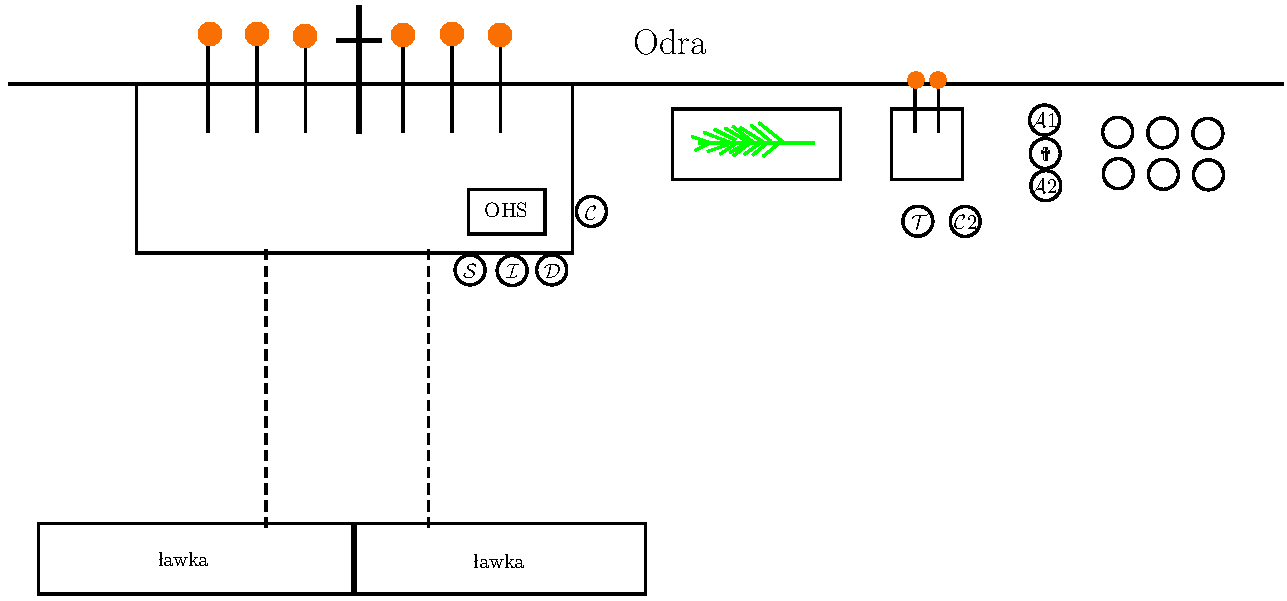
\includegraphics[width=\linewidth]{Palmowa/PalmyNadOdra.pdf}
			\caption{Ustawienie po przyjściu do ołtarza}
		\end{figure}
	
		\bigskip
	
		\begin{itemize}
			\item \ii~ cicho odczytuje antyfonę \textit{Hosanna filio David}, tak jak podczas Mszy, a następnie śpiewa \textit{Dominus vobiscum}, zwrócony w kierunku księgi,
			\item po \textit{Amen} następuje zasypanie, 
			\item \aa1 podaje wodę \cc~ a ten podaje ją \dd,
			\item następuje pokropienie, \aa1 odbiera wodę od \dd,
			\item następuję okadzenie,
			\item palmę dla \ii~ \dd~ kładzie na ołtarzu,
			\item następuje rozdawanie palm (\cc2 podaje palmy, \cc1 zawiaduje ruchem), odbieranie palm od \ii~ z pocałunkiem, asysta ustawia się dwójkami jak do komunii w kolejności: lewici, klerycy, ministranci, lud,
			\item po rozdaniu palm \ii~ myje ręce, pomagają mu w tym \aa,
			\item następuje odśpiewanie ewangelii, nie przenosi się mszału,
			\item do ewangelii ustawiamy się jak podczas mszy, gdy już dojdziemy na miejsce jak na Rys 2, 
	
		\begin{figure}[h!]
			\centering
			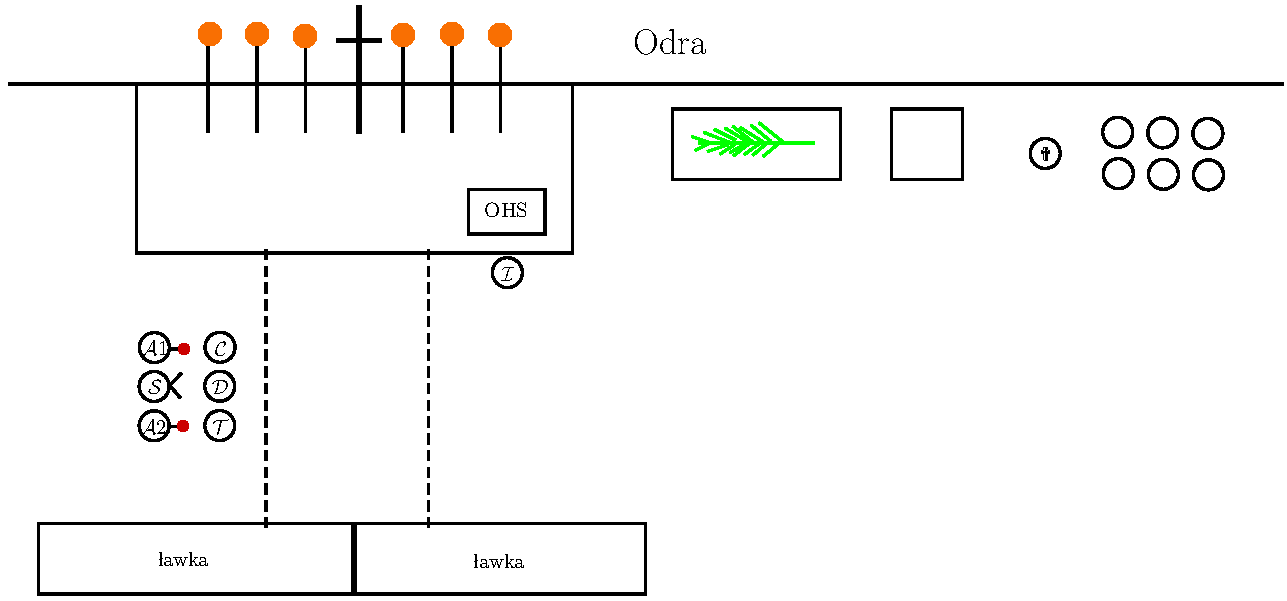
\includegraphics[width=\linewidth]{Palmowa/PalmyNadOdra2.pdf}
			\caption{Ustawienie podczas Ewangelii}
		\end{figure}
		
			\item po odśpiewaniu ewangelii \ii~ całuje ewangeliarz oraz jest okadzany przez \dd,
			\item kantorzy ($A$) oraz mikrofoniarz udają się najkrótszą możliwą drogą do pierwszych drzwi kościoła. Przymykają je lekko, ale obserwują, czy procesja już się zbliża. Dwóch lub jeden Kantor ($B$) pozostaje w procesji z ministrantami,
			\item po powrocie do pozycji z Rys 1 następuje zasypanie,
			\item lewici stają w rzędzie za	\ii,
			\item \dd~ staje obok rzędu i śpiewa \textit{Procedeamus in pace},
			\item Kantor ($B$) oraz mikrofon wraz z ludem śpiewa \textit{In nomine Christi. Amen}, a następnie rozpocznie jedno z poniższych: 
			
			\begin{itemize}
				\item śpiew jednej z antyfon procesyjnych z \textit{Liber Usualis},
				\item \textit{Christus vincit},
				\item pieśń po polsku do Chrystusa Króla;
			\end{itemize}

			\item po oddaniu rewerencji ołtarzowi \cc~ oddaje nakrycia głowy,
			\item ustawiamy się w szyku procesyjnym, Kantor/Kantorzy ($B$) zajmują w procesji miejsce zaraz za \ding{63},
			\item udajemy się w kierunku bocznych drzwi po schodach za pomnikiem biskupa Kominka,
			\item kantorzy A wewnątrz kościoła obserwują delikatnie, czy procesja nadchodzi,
			\item kiedy procesja dochodzi do drzwi Kościoła, \ss~ z \aa~ stają przodem do drzwi, a ministranci rozchodzą się na boki tworząc szpaler tak aby \ii~ znajdował się nieopodal \ding{63}, jak na Rys 3,
			
			\bigskip
			
			\begin{figure}[h]
				\centering
				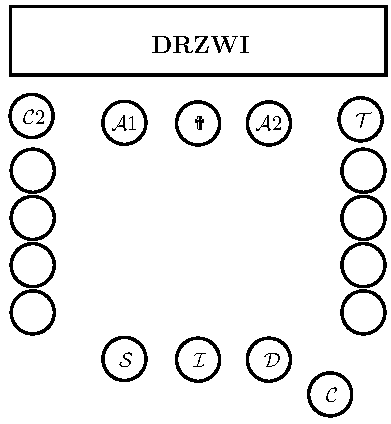
\includegraphics[width=0.26\linewidth]{Palmowa/PalmyNadOdra3.pdf}
				\caption{Procesja przy drzwiach kościoła}
			\end{figure}
			
			\item kantorzy ($A$) (w środku) stojąc zwróceni w kierunku drzwi śpiewają: \textit{Gloria Laus et honor} etc.,
			\item kantorzy ($B$), ministranci i wierni powtarzają werset: \textit{Gloria Laus},
			\item kantorzy ($A$) śpiewają poszczególne zwrotki hymnu, po każdej zwrotce Kantorzy ($B$) + reszta odśpiewują refren: \textit{Gloria, Laus},
			\item po piątej zwrotce i refrenie \ding{63} głośno i widocznie uderza nóżką krzyża procesyjnego w drzwi, a Kantorzy ($A$) i \cc2 szeroko otwierają drzwi,
			\item \cc2 wprowadza \ding{63} i resztę procesji do wnętrza kościoła. W tym czasie Kantorzy ($A$) i Kantorzy ($B$) łączą się w jedną grupę i jak najszybciej zaczynają śpiew: \textit{Ingrediente Domino}, podany w \textit{Liber Usualis};
			\item \dd~, \ss~, \ii~ oraz \cc~ po przyklęknięciu na środku udają się bezpośrednio do księgi po stronie epistoły, reszta asysty i chór przyklękają po kolei na środku. Wszyscy zajmują swoje miejsca i odkładają palmy. \aa~ odkładają świece a \ding{63} krzyż 
			\item modlitwa na zakończenie procesji od Mszału ustawionego przy ołtarzu po stronie Epistoły, lewici trzymają brzegi kapy (jak przy poświęceniu),
			\item po skończonej oracji, \ii~ i \dd~ oraz \ss~ podchodzą do sedilli i przebierają się. Przebieranie przebiega w następującej kolejności:
			
			\begin{itemize}
				\item \cc~ zabiera kapę przekazuje zakrystianom,
				\item lewici ściągają dalmatyki z pomocą \aa1 oraz \aa2 i \cc,
				\item lewici ubierają w ornat \ii, zakrystianie zabierają w tym czasie dalmatyki i manipularze czerwone
				\item \aa1 zakłada tunicelę \ss, \aa2 dalmatykę \dd,
				\item \cc~ sprawdza czy \dd~ i \ss~ mają swoje szaty
			\end{itemize}
			
		\end{itemize}
	
	\enlargethispage{20pt}
	
%	\section{Poświęcenie palm}
%
%		\begin{itemize}
%		  \item wszyscy procesyjnie udają się do ołtarza w kolejności:
%		  
%		    \begin{enumerate}\centering
%		     \item[] $\mathcal{T}$~~~$\mathcal{C}2$
%		     \item[] $\mathcal{A}1$~~~\ding{63}~~~$\mathcal{A}2$ 
%		     \item[] reszta chóru parami
%		     \item[] $\mathcal{C}1$
%		     \item[] $\mathcal{S}$~~~$\mathcal{I}$~~~$\mathcal{D}$
%		    \end{enumerate}
%		    
%		    \item po przklęknięciu wszyscy udają się na swoje miejsca -- chór \textbf{stoi}
%		    \item \sout{$\mathcal{A}1$ i $\mathcal{A}2$ zanoszą stolik z palmami na środek prezbiterium} stolik jest już wyniesiony
%		    \item $\mathcal{I}$ z $\mathcal{D}$ i $\mathcal{S}$ udają się do stolika z palmami (twarzą do ludzi)
%		    \item $\mathcal{T}$ i $\mathcal{C}2$ stają przy stoliku po stronie Ewangelii, a $\mathcal{C}1$ - Epistoły
%		    
%		    \begin{figure}[h]
%		      \centering
%		      
\includegraphics[scale=3]{Palmy.eps}
%		    \end{figure}
%		    
%		    \item następuje błogosławieństwo, pokropienie palm, zasypanie kadzidła i okadzenie palm \footnote{Małaczyński s. 59-60}
%		    \item $\mathcal{I}$ z $\mathcal{D}$ i $\mathcal{S}$ idą do ołtarza, a chór ustawia się parami tak, jak do Komunii
%		    
%		    %\newpage
%		    
%		    \item palmy odbierane są przez ministrantów parami w sposób następujący:
%		      \begin{enumerate}[leftmargin=1cm]
%		       \item przyklęknięcie na posadzce
%		       \item wejście po stopniach i uklęknięcie na ostatnim
%		       \item odebranie palmy \textbf{z pocałunkiem} w dłoń $\mathcal{I}$
%		       \item powstanie, przyklęknięcie w miejscu i udanie się w swoje miejsce
%		      \end{enumerate}
%		    \item $\mathcal{I}$ z $\mathcal{D}$ i $\mathcal{S}$ rozdają palmy ludowi -- chór \textbf{siada}
%		    \item $\mathcal{A}1$ i $\mathcal{A}2$ zabierają stół z palmami, gdy kończy się ich rozdawanie
%		    \item $\mathcal{A}1$ i $\mathcal{A}2$ asystują przy obmyciu rąk $\mathcal{I}$ (przy kredensji)
%		    \item $\mathcal{I}$ z $\mathcal{D}$ i $\mathcal{S}$ idą do ołtarza, a tam następuje zasypanie kadzidła
%		    
%		    \newpage
%		    
%		    \item formuje się procesja do Ewangelii (patrząc od ołtarza):
%		      \begin{enumerate}\centering
%		       \item[] (stopnie ołtarza)
%		       \item[] $\mathcal{S}$~~~$\mathcal{D}$
%		       \item[] $\mathcal{C}$1~~~$\mathcal{T}$
%		       \item[] $\mathcal{A}$2~~~$\mathcal{A}$1
%		      \end{enumerate}
%		    \item na znak ceremoniarza formacja klęka i udaje się w wyznaczone miejsce
%		    
%		    \begin{figure}[h]
%		      \centering
%		      
\includegraphics[scale=3]{Ewangelia.eps}
%		    \end{figure}
%		    
%		    {\color{Red} \item chór na czas Ewangelii wstaje i obraca się w twarzą do \underline{\textbf{\color{Red}Ewangeliarza}} (i w tamtym kierunku wykonuje wszystkie skłony przepisane)}
%		    \item po Ewangeli $\mathcal{S}$ i $\mathcal{C}1$ udają się do $\mathcal{I}$
%		    \item $\mathcal{A}$1 i $\mathcal{A}$2 idą na środek prezbiterium (przy balaskach) i tam czekają 
%		    \item $\mathcal{D}$ i $\mathcal{T}$ udają się do ołatarza, żeby zasypać kadzidło
%		  \end{itemize}
%
%	\section{Procesja z palmami}
%
%		\begin{itemize}
%		 \item następuje zasypanie przy ołtarzu
%		 \item w międzyczasie formuje się procesja (kolejność taka sama, jak przy wejściu)
%		 \item podczas śpiewania \textit{Procedamus in pace} $\mathcal{I}$ ,$\mathcal{D}$ i $\mathcal{S}$ stoją jeden za drugim
%		 \item na znak $\mathcal{C}1$ ministranci klękają (oprócz $\mathcal{A}1$, $\mathcal{A}2$ i \ding{63}) i rusza prosceja prowadzona przez $\mathcal{C}2$ 
%		 \item po dojściu do stopni ołtarza, ministranci przyklękają parami i udają się na swoje miejsca, a chór stoi
%		 \item $\mathcal{C}2$ zanosi na ołtarz Mszał i stawia go po stronie Epistoły
%		 \item $\mathcal{I}$ z $\mathcal{D}$ i $\mathcal{S}$ przyklękają i udają się po skosie na stronę Epistoły (stają jeden za drugim)
%		 \item $\mathcal{I}$ śpiewa \textit{Dominus Vobiscum} bez odwracania się do ludu \footnote{Część współczesnych liturgistów zajmujących się klasycznym rytem zwraca uwagę na to, iż odmawianie modlitw versus populum, pomimo iż jest zawarte w rubrykach OHS, nie stanowi integralnej części rytu rzymskiego z 1962, lecz było wdrażanych jako część „uproszczonego rytu zreformowanego z 1965”. Zalecają zastosowanie w przypadku tych modlitw analogicznych rozwiązań z innych dni liturgicznych lub sprzed reformy Wielkiego Tygodnia. Poniższe rozwiązanie nawiązuje do oracji przy poświęceniu popiołu w Środę popielcową. Źródło: Cykl wykładów wygłoszonych przez ks. Svena Conrada FSSP w Wigratzbad w marcu 2015r.}
%		 \item po zaśpiewanej przez $\mathcal{I}$ oracji, udaje się on wraz z $\mathcal{D}$ i $\mathcal{S}$ krótką drogą do sedilii
%		 \item $\mathcal{I}$ z $\mathcal{D}$ i $\mathcal{S}$ zmieniają szaty, a pomagają im $\mathcal{A}1$, $\mathcal{A}2$, $\mathcal{C}1$
%		\end{itemize}

	\section{Msza Święta - ważniejsze zmiany}
		\begin{itemize}
		 \item wszyscy odkładają palmy
		 \item nie odmawia się modlitw u stopni
		 \item bezpośrednio po przyklęknięciu następuje ucałowanie ołtarza i nałożenie kadzidła
		 \item po odmówieniu \textit{Introitu} i \textit{Kyrie} $\mathcal{I}$ i $\mathcal{D}$ oraz $\mathcal{S}$ krótką drogą schodzą do sedilii
		 \item podczas lekcji na słowa \textit{in nomine Iesu omne genu flectatur} wszyscy przyklękają
		 \item procesja przed Ewanglią, jak i funkcje tworzących ich ministrantów pozostają (prawie) bez zmian względem Mszy śpiewanej (za wyjątkiem nietrzymania w jej czasie paramentów litrugicznych); więcej patrz \hyperref[E]{Dodatek}
		 \item chór podczas Ewangelii wykonuje skłony w kierunku krzyża ołtarzowego, a śpiewacy ``przed siebie``
		 \item po przyjęciu przez $\mathcal{I}$ Komunii Św. i wyciągnięciu puszki z tabernakulum $\mathcal{D}$ \textbf{sam} odmawia \textit{Confiteor}, po którym nastepuje \textit{Misereatur} -- \textbf{wszyscy} są w tym czasie pochyleni. Prostujemy się dopiero na \textit{Indulgenciam}
		 \item nie ma ostatniej Ewangelii
		
		\end{itemize}

\section{Dodatek}
	  \subsection{Losy subdiakona krucyfera}
	    \begin{itemize}
	    \item subdiakon krucyfer ( \ding{63} ), ubrany w albę, cingulum i czerwoną tunicellę 
	    \item nie odbiera palmy od $\mathcal{I}$. 
	    \item po skończonej procesji idzie do kaplicy zimowej, gdzie ściąga westymenta subdiakona, zakłada komżę, bierze biret i przechodzi do chóru.
	    \end{itemize}
    
  %\newpage
  
  \subsection{Prosecja do Ewangelii - dla zaawansowanych}
  \label{E}
    \subsubsection*{\textbf{Celebrans z subdiakonem i ceremoniarzem }}
      \begin{itemize}
      \item kiedy skończy się śpiew Graduału i Traktusa, $\mathcal{I}$ wraz z $\mathcal{S}$ i $\mathcal{C}1$ podchodzą do ołtarza - przyklękają 
      \item $\mathcal{I}$ wchodzi na najwyższy stopień i odmawia modlitwę \textit{Munda cor} 
      \item \ss~ w tym czasie przenosi mszał,
      \end{itemize}
      
    \subsubsection*{\textbf{Diakon}}
      \begin{itemize}
       \item przy pomocy $\mathcal{C}2$ zdejmuje dalmatykę i manipularz 
       \item od $\mathcal{C}2$ otrzymuje księgę z tekstem Pasji, a następnie zajmuje miejsce pomiędzy dwoma śpiewakami - $\mathcal{S}1$ i $\mathcal{S}2$
      \end{itemize}
      
    \subsubsection*{\textbf{Ale jak to wygląda?}}

    \begin{enumerate}\centering
     \item[] $\mathcal{I}$
     \item[] (stopnie ołtarza)
     \item[] $\mathcal{S}$
     \item[] 
     \item[] 
     \item[] $\mathcal{S}1$~~~$\mathcal{D}$~~~$\mathcal{S}2$
     \item[] $\mathcal{C}2$
    \end{enumerate}
    
   % \newpage
    
    \begin{itemize}
     \item na znak $\mathcal{C}2$ wszyscy oprócz $\mathcal{I}$ przyklękają 
     \item $\mathcal{S}$ przechodzi ze Mszałem na stronę Ewangelii i pozostaje przy nim asystując $\mathcal{I}$ przy kartkach 
     \item $\mathcal{C}1$, $\mathcal{T}$, $\mathcal{A}1$, $\mathcal{A}2$ \textbf{nie} ustawiają się jak na Mszy śpiewanej (zostają na swoich 'bazach') i skłaniają się do krzyża ołtarzowego razem z $\mathcal{I}$ \footnote{Ceremoniał o. Małaczyńskiego, str. 65, pkt. 47(dla rytu uroczystego): „Jeżeli Męka Pańska nie jest śpiewana celebrans pod koniec traktusa odmawia „Munda cor” i czyta Mękę Pańską po stronie Ewangelii. Równocześnie należy ją odczytać wiernym  po polsku."}
     \item[]
     \item $\mathcal{C}2$ prowadzi $\mathcal{S}1$, $\mathcal{D}$, $\mathcal{S}2$ do ambony – gdzie następuje śpiew Pasji po polsku
     \item wszystkie skłony podczas Pasji wykonujemy w stronę ewangeliarza/lekcjonarza (nie w stronę Mszału),
     \item[]
     \item po odśpiewanej Pasji po polsku $\mathcal{I}$ staje przed środkiem ołtarza, a $\mathcal{S}$ za nim na swoim stopniu. 
     \item $\mathcal{D}$, $\mathcal{S}1$, $\mathcal{S}2$ i $\mathcal{C}2$ przyklękają na środku, po czym $\mathcal{C}2$ prowadzi $\mathcal{D}$ do sedilli i pomaga mu założyć dalmatykę i manipularz 
     \item $\mathcal{D}$ zajmuje swoje miejsce za $\mathcal{I}$ i przyklęka -- $\mathcal{I}$ rozpoczyna \textit{Credo}
    \end{itemize}

%  \section{Do poprawy}
%    \begin{itemize}
%     \item {\color{red}Przypomnieć ministrantom, żeby na Ewangelie skłaniali głowy \textbf{do Ewangeliarza}, a nie do ołtarza.}
%     \item \sout{Jeśliby dobrze poukładać palmy na stoliku, tak żeby całość była stabilna, to można by się pokusić o 'wjechanie' nim na środek jak już przejdzie cała procesja.}
%    \end{itemize}

% \newpage

% %\chapter{}

\section{Sposoby służenia na Piasku}

\subsection{Rodzaje Mszy Św.}

\begin{itemize}
	\item \textbf{recytowana} -- z jednym lub dwoma ministrantami
	\item \textbf{recytowana świąteczna} (także kolędowa) -- z jednym lub dwoma,
	      w niedziele i święta poza wielkim postem, klęczy się na niej i stoi
	      jak na mszy śpiewanej
	\item \textbf{śpiewana \textit{na dwóch}} -- msza śpiewana bez \cc~ i \tt~
	\item \textbf{śpiewana z okadzeniem} -- standardowa msza niedzielna z \cc~ i
	      \tt~
	\item \textbf{ śpiewana \textit{bardziej uroczysta}} -- bardziej uroczysta
	      msza świąteczna	(np. Wigilia Zesłania Ducha Św.), z lucenarium,
	      obrusem komunijnym, okadzeniem i ew. dodatkowymi obrzędami
	\item \textbf{solenna} -- z asystą \dd~ i \ss, lucenarium
\end{itemize}

\noindent Przy zastosowaniu bardziej uroczystych form liturgicznych -- jeśli
jest duża ilość ministrantów -- wyznacza się drugiego ceremoniarza, który
\begin{itemize}
	\item prowadzi procesję wejścia i inne procesje, które także ustawia przed
	      wyruszeniem. Dba o dobre tempo
	\item wprowadza duchownych i ministrantów do chóru
	\item w razie potrzeby zajmuje miejsce przy \cc1, aby wspólnie asystować
	      \ii.
	\item kontroluje na bieżąco, czy czegoś nie brakuje, czy nie powinien czegoś
	      donieść itp.
	\item wprowadza lucenarium i procesję „dwójkami” do przyjmowania Komunii Św.
\end{itemize}


% \section{Poświęcenie palm i procesja}

\begin{itemize}
	\item w tej części \dd~ wykonuje pocałunki \ii~ standardowo jak podczas mszy
	\item podczas ubierania (na {\color{red} czerwono}) celebransa asystuje \cc,
	      kolejno diakona \aa1 oraz subdiakona \aa2
	\item ustawiamy się w szyku procesyjnym. \dd~ i \ss~ przez cały czas
	      procesji i poświęcenia ,jeżeli jest to możliwe, trzymają kapę.
	      Wychodzimy przez główne wyjście na zewnątrz. Przy przechodzeniu przez
	      oś ołtarza polowego, przyklękają wszyscy oprócz: \ding{63}, \aa1, \aa2
	      oraz \ii
	\item schola śpiewa podczas procesji \textit{Hosanna filio David} na
	      przemian z Psalmem 117 \footnote{Zob. \textit{Liber Usualis} z 1961 :
		      Ritus servandus in celebratione Missae in Cantu ad 1.}
	\item po dojściu na miejsce święcenia palm, \cc~ odbiera nakrycia głowy,
	      następuje  oddanie referencji ołtarzowi przez \dd~ i \ss~ oraz \ii~
	      (\dd~ i \ss~ przyklękają, \ii~ głęboko się skłania), \ii~ całuje
	      ołtarz następnie ustawiamy się w sposób przedstawiony na Rys.
	      \ref{fig:przyjscie}

	      \begin{figure}[h]
		      \centering
		      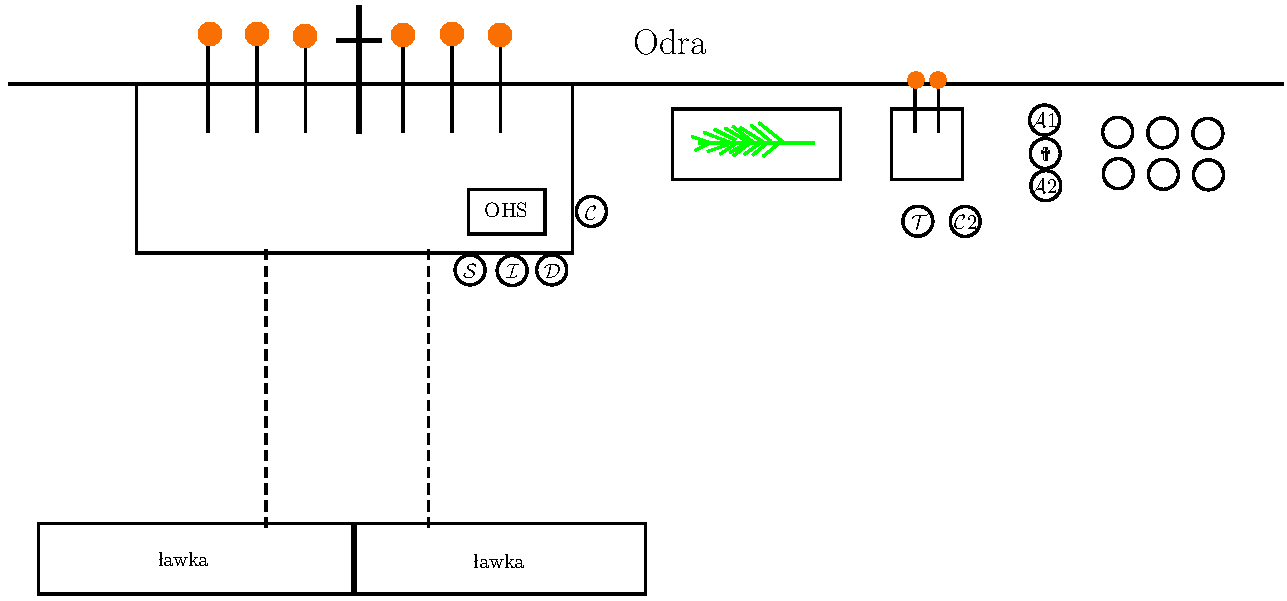
\includegraphics[width=0.8\linewidth]{Palmowa/PalmyNadOdra.pdf}
		      \caption{Ustawienie po przyjściu do ołtarza}
		      \label{fig:przyjscie}
	      \end{figure}

	\item \ii~ cicho odczytuje antyfonę \textit{Hosanna filio David}, tak jak
	      podczas Mszy, a następnie śpiewa \textit{Dominus vobiscum}, zwrócony w
	      kierunku księgi
	\item po \textit{Amen} następuje zasypanie
	\item \aa1 podaje wodę \cc~ a ten podaje ją \dd
	\item następuje pokropienie, \aa1 odbiera wodę od \dd
	\item następuję okadzenie
	\item palmę dla \ii~ \dd~ kładzie na ołtarzu
	\item następuje rozdawanie palm (\cc2 podaje palmy, \cc1 zawiaduje ruchem),
	      odbieranie palm od \ii~ i \dd~ z pocałunkiem, asysta ustawia się
	      dwójkami jak do komunii w kolejności: \dd~ i \ss~, klerycy,
	      ministranci, lud
	\item po rozdaniu palm \ii~ i \dd~ myją ręce, pomagają mu w tym \aa\aa
	\item następuje odśpiewanie ewangelii, nie przenosi się mszału
	\item do ewangelii ustawiamy się jak podczas mszy, gdy już dojdziemy na
	      miejsce jak na Rys. \ref{fig:ewangelia}

	      \begin{figure}[h!]
		      \centering
		      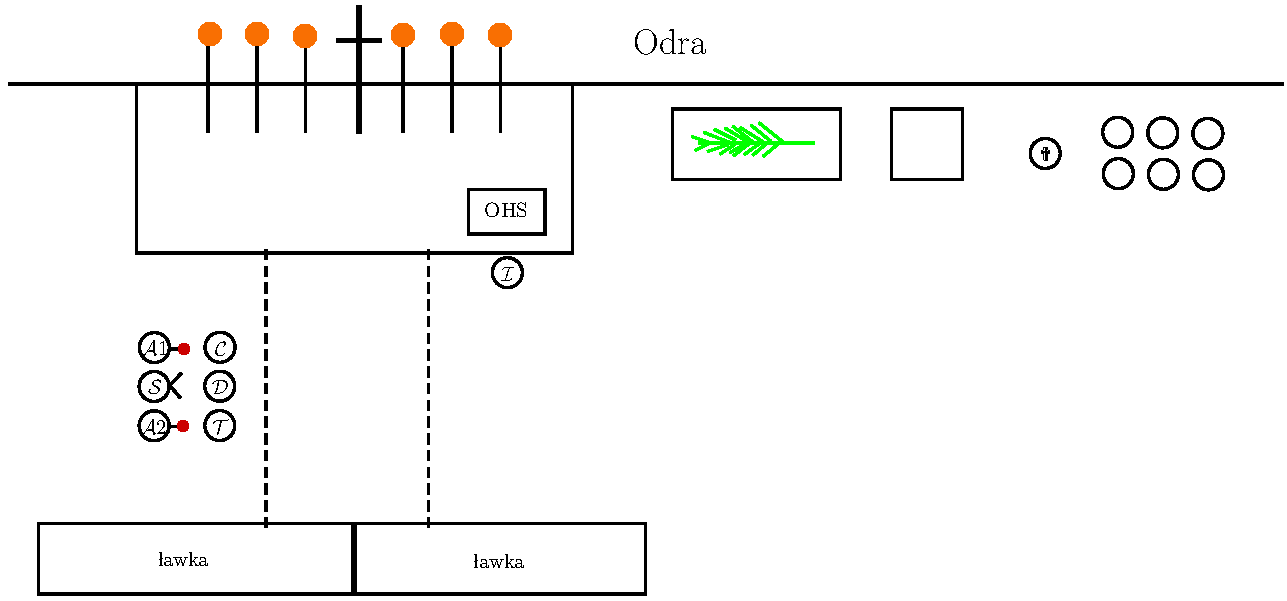
\includegraphics[width=0.8\linewidth]{Palmowa/PalmyNadOdra2.pdf}
		      \caption{Ustawienie podczas Ewangelii}
		      \label{fig:ewangelia}
	      \end{figure}

	\item po odśpiewaniu ewangelii \ii~ całuje ewangeliarz oraz jest okadzany
	      przez \dd
	\item kantorzy ($K1$) oraz mikrofoniarz udają się najkrótszą możliwą drogą
	      do pierwszych drzwi kościoła. Przymykają je lekko, ale obserwują, czy
	      procesja już się zbliża. Dwóch lub jeden kantor ($K2$) pozostaje w
	      procesji z ministrantami
	\item po powrocie do pozycji z Rys. \ref{fig:przyjscie} następuje zasypanie
	\item \dd~ i \ss~ stają w rzędzie za \ii
	\item \dd~ staje obok rzędu i śpiewa \textit{Procedeamus in pace}
	\item kantor ($K2$) oraz mikrofon wraz z ludem śpiewa \textit{In nomine
		      Christi. Amen}, a następnie rozpocznie jedno z poniższych:

	      \begin{itemize}
		      \item śpiew jednej z antyfon procesyjnych z \textit{Liber
			            Usualis}
		      \item \textit{Christus vincit}
		      \item pieśń po polsku do Chrystusa Króla
	      \end{itemize}

	\item po oddaniu rewerencji ołtarzowi \cc~ oddaje nakrycia głowy
	\item ustawiamy się w szyku procesyjnym, $K2$ zajmują w procesji miejsce
	      zaraz za \ding{63}
	\item udajemy się w kierunku bocznych drzwi po schodach za pomnikiem biskupa
	      Kominka
	\item $K1$ wewnątrz kościoła obserwują delikatnie, czy procesja nadchodzi
	\item kiedy procesja dochodzi do drzwi kościoła, \ss~ z \aa\aa~ stają przodem
	      do drzwi, a ministranci rozchodzą się na boki tworząc szpaler tak aby
	      \ii~ znajdował się nieopodal \ding{63}, jak na Rys. \ref{fig:procesja}

	      \medskip

	      \begin{figure}[h]
		      \centering
		      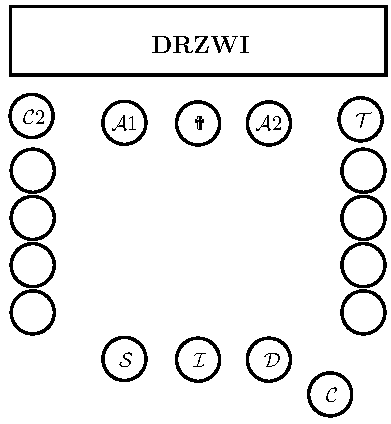
\includegraphics[width=0.26\linewidth]{Palmowa/PalmyNadOdra3.pdf}
		      \caption{Procesja przy drzwiach kościoła}
		      \label{fig:procesja}
	      \end{figure}
	      \todo{A gdzie mają być ci kantorzy na tym rysunku?}

	\item $K1$ (w środku) stojąc zwróceni w kierunku drzwi śpiewają:
	      \textit{Gloria Laus et honor} etc.
	\item $K2$, ministranci i wierni powtarzają werset: \textit{Gloria Laus}
	\item $K1$ śpiewają poszczególne zwrotki hymnu, po każdej zwrotce
	      $K2$ i reszta odśpiewują refren: \textit{Gloria, Laus}
	\item po piątej zwrotce i refrenie \ding{63} głośno i widocznie uderza nóżką
	      krzyża procesyjnego w drzwi, a $K1$ i \cc2 szeroko otwierają drzwi
	\item \cc2 wprowadza \ding{63} i resztę procesji do wnętrza kościoła. W tym
	      czasie $K1$ i $K2$ łączą się w jedną grupę i jak najszybciej zaczynają
	      śpiew: \textit{Ingrediente Domino}, podany w
	      \textit{Liber Usualis}
	\item \dd, \ss, \ii~ oraz \cc~ po przyklęknięciu na środku udają się
	      bezpośrednio do księgi po stronie epistoły, reszta asysty i chór
	      przyklękają po kolei na środku. Wszyscy zajmują swoje miejsca i
	      odkładają palmy. \aa\aa~ odkładają świece a \ding{63} krzyż na stojak
	\item modlitwa na zakończenie procesji od Mszału ustawionego przy ołtarzu po
	      stronie Epistoły, \dd~ i \ss~ trzymają brzegi kapy (jak przy poświęceniu)
	\item po skończonej oracji, \ii~ i \dd~ oraz \ss~ podchodzą do sedilli i
	      przebierają się (w {\color{violet}fiolety}). Przebieranie przebiega w
	      następującej kolejności:

	      \begin{itemize}
		      \item \cc~ zabiera kapę przekazuje \zz
		      \item \dd~ i \ss~ ściągają dalmatyki z pomocą \aa1 oraz \aa2
		      \item \cc~ ubierają w ornat \ii, \zz~ zabierają w tym
		            czasie dalmatyki i manipularze czerwone
		      \item \aa1 zakłada tunicelę \ss, \aa2 dalmatykę \dd
		      \item \cc~ sprawdza czy \dd~ i \ss~ mają odpowiednie szaty
	      \end{itemize}

	\item w czasie przebierania schola śpiewa \textit{Introit}
\end{itemize}

% \section{Liturgia słowa}

\begin{itemize}
	\item po przybyciu do prezbiterium stajemy następująco:
	\item (tutaj będzie grafika)
	\item następuje zasypanie, potem \cc~ odmawia modlitwę, okadzenie księgi i
	      \textit{Exsultet}
	\item \aa~ biorą z kredensu świeczki i odpalają sobie, podobnie \mm1
	\item \cc2 na słowa \textit{O vere beata nox...} zapala lampy w
	      prezbiterium.
	\item po orędziu paschalnym \cc2 wraz z \aa2 pomagają \ii~ przebrać się z
	      powrotem w kapę
	\item następnie \cc~ odnosi dalmatykę do zakrystii i wraca na swoje miejsce
	      razem z drugim OHS
	\item \cc1 zabiera z pulpitu białą narzutkę i kładzie na pulpicie teksty
	      proroctw
	\item \ding{63} odnosi krzyż za ołtarz
	\item \tt~ odnosi kadzielnicę i wraca na swoje miejsce
	\item siedzimy w prezbiterium następująco:
	\item (tutaj będzie odpowiednia grafika)
	\item następują proroctwa
	\item po trzecim proroctwie \tt~ idzie po kadzielnicę i bokiem przemyka w
	      stronę chrzcielnicy i zapala tam światła
\end{itemize}

% \section{Lucenarium}

\opis{Potrzebne: 6(4) ministrantów siedzących w chórze, \cc2 lub \tt~ (gdy nie
	ma \cc2 \tt~ prowadzi i daje znaki), 6(4) pochodni wystawionych koło bazy \tt}

\begin{itemize}
	\item Po okadzeniu ludu \tt~ zatrzymuje się n przy stopniu prezbiterium i
	      zwraca się w kierunku ołtarza. Dołącza do niego \cc2 i 6 ministrantów
	      wyznaczonych do lucenarium.
	\item Na znak \cc2 klękają i wychodzą do bocznej nawy po pochodnie.	(Rys.
	      \ref{fig:wyjscie})
	\item Przygotowują pochodnie, mogą zasypać kadzielnicę.
	\item Na śpiew \textit{Sanctus} bardzo powoli wchodzą do prezbiterium
	      rozchodząc się na boki (Rys.\ref{fig:wejscie_1})
	\item Ustawieni odpowiednio przyklękają, po czym klękają na dwa kolana
	      (Rys.\ref{fig:wejscie_2})
	\item \tt~ zajmuje miejsce z prawej strony na pierwszym stopniu ołtarza.
	      Klęczą przez cały Kanon.
	\item Na \textit{Per omnia saecula saeculorum} wstają, wykonują skłon na
	      \textit{Oremus}, a następnie przyklękają i na czele z \tt~ i \cc2
	      wychodzą z prezbiterium (Rys. \ref{fig:wyjscie_1} oraz Rys.
	      \ref{fig:wyjscie_2})
\end{itemize}

\begin{figure}[h]
	\centering
	\includegraphics[width=0.29\linewidth]{wyjscie}
	\caption{Wyjście ministrantów podczas ofiarowania}
	\label{fig:wyjscie}
\end{figure}

\begin{figure}[ht]
	\savebox{\imagebox}{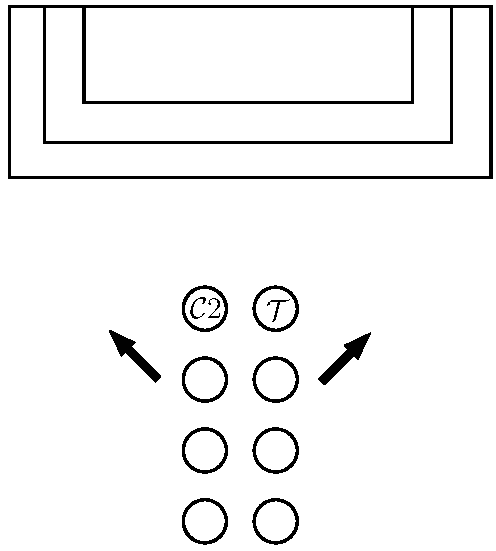
\includegraphics[width=.4\linewidth]{wejscie_1}}%
	\begin{subfigure}[t]{.5\linewidth}
		\centering\usebox{\imagebox}
		\caption{Przed przyklęknięciem}
		\label{fig:wejscie_1}
	\end{subfigure}\qquad
	\begin{subfigure}[t]{.5\linewidth}
		\centering\raisebox{\dimexpr\ht\imagebox-\height}{% Raise smaller image
			into place \includegraphics[width=\linewidth]{wejscie_2}}%
		\caption{Po przyklęknięciu}
		\label{fig:wejscie_2}
	\end{subfigure}
	\caption{Wejście ministrantów na \textit{Sanctus}}
\end{figure}

\newpage

\begin{figure}[ht]
	\savebox{\imagebox}{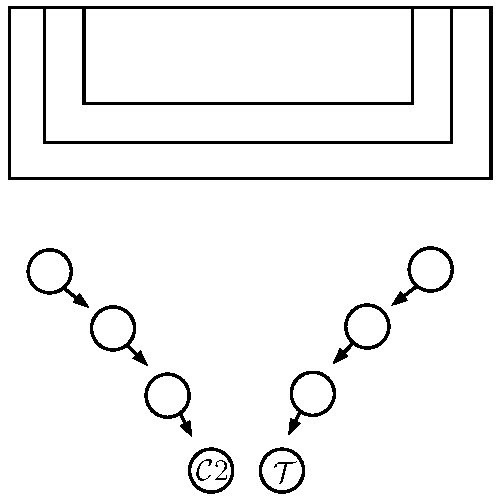
\includegraphics[width=.4\linewidth]{wyjscie_2}}%
	\begin{subfigure}[t]{.5\linewidth}
		\centering\raisebox{\dimexpr\ht\imagebox-\height}{% Raise smaller image
			into place 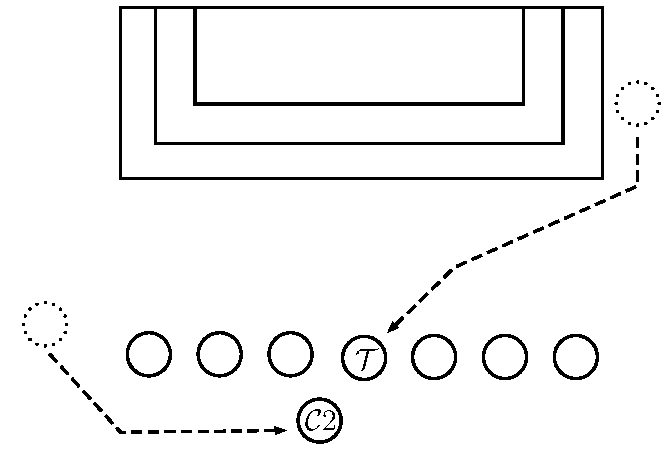
\includegraphics[width=\linewidth]{wyjscie_1}}%
		\caption{Przed przyklęknięciem}
		\label{fig:wyjscie_1}
	\end{subfigure}\qquad
	\begin{subfigure}[t]{.5\linewidth}
		\centering\usebox{\imagebox}
		\caption{Po przyklęknięciu}
		\label{fig:wyjscie_2}
	\end{subfigure}
	\caption{Wyjście ministrantów po \textit{Per omnia secula seculorum}}
\end{figure}

\textbf{Uwaga!} Na Mszy Wieczerzy Pańskiej w Wielki Czwartek ministranci z
pochodniami nie wychodzą z prezbiterium, tylko oczekują na procesję.

% \section{Dodatek}

\subsection{Przebieg poświęcenia wody}
\label{sec:woda}
\begin{enumerate}
      \item \textit{Dominus Vobiscum} i Oracja 0. (przed wejściem)
            \smallfont{(złożone ręce)}
      \item \textit{Dominus Vobiscum} i Oracja 1. \smallfont{(złożone ręce)}
      \item Prefacja do słów \textit{Sumat unigeniti tui gratiam de Spiritu
                  Sancto}
      \item \ii~ kreśli znak krzyża
            \textcolor{red}{\raisebox{-1mm}{\scalebox{1.5}{\ding{64}}}} na
            wodzie
      \item Wyciera ręce
      \item Kontynuuje modlitwę
      \item Na \textit{Sit haec} kładzie rękę na powierzchni wody
      \item Wyciera rękę
      \item Kreśli znaki krzyża
            \textcolor{red}{\raisebox{-1mm}{\scalebox{1.5}{\ding{64}}}}
            nad wodą na słowa \textit{Per Deum vivum \dots}
            \vspace*{-11pt}
      \item Wylewa wodę na cztery strony świata po słowach \textit{... super te
                  ferebatur} ~~~
            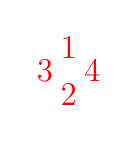
\begin{tikzpicture}[scale=0.3, baseline=-1mm, thick]
                  \draw[color=red] (10mm,0) node {\large 4};
                  \draw[color=red] (-10mm,0) node {\large 3};
                  \draw[color=red] (0,10mm) node {\large 1};
                  \draw[color=red] (0,-10mm) node {\large 2};
            \end{tikzpicture}
            \vspace*{-7pt}
      \item Kreśli znak krzyża nad wodą na \textit{Benedico te}
      \item Po zmianie głosu na \textit{recto tono} na słowa \textit{tu benignus
                  aspira} trzy razy dmucha do wody na kształt krzyża
      \item W tym czasie \cc1 podaje Paschał
      \item Na słowa \textit{Descendad in hanc} trzy razy wkłada Paschał do wody
            i śpiewa \footnote{Wkłada Paschał coraz głębiej}
      \item \ii~ trzy razy dmucha do wody w kształcie litery
            \textcolor{red}{\raisebox{-1mm}{\Large ${\Psi}$}} i kontynuuje
            \textit{Totamque ... effectu}
      \item Wyciągamy Paschał z wody i kończymy święcenie wody (\textit{... per
                  ignem.})
      \item Po \textit{Amen} nabiera się wody do pokropienia
      \item Pokropienie i \textit{Com przyrzekł Bogu \dots}
      \item Następnie \cc1 przynosi do chrzcielnicy tackę z olejami świętymi i
            wręcza \ii~ (z pocałunkiem) odpowiednie ampułki. \ii, wypowiadając
            słowa przepisane w księdze po kolei:
            \begin{itemize}
                  \item wlewa olej katechumenów
                  \item wlewa krzyżmo
                  \item wlewa oba
            \end{itemize}
      \item Następnie miesza wodę ręką lub przy pomocy łyżeczki \footnote{W
                  razie potrzeby myje i wyciera ręce; wykorzystuje sól, watę i
                  miękisz chleba, które później należy spalić. Wodę z tej
                  ablucji wlewa się do sacrarium.}
\end{enumerate}

\subsection{Bierzmowanie}
\label{sec:bierz}
\begin{enumerate}
      \item \dd~ i \ss~ podtrzymują kapę; księgę trzyma \cc1, a \cc2 stoi z boku
            przy kredencji
      \item \ii~ zwraca się do kandydatów \textit{Spiritus
                  Sanctus superveniat\dots Amen.}
      \item \ii~ żegna się mówiąc \textit{Adjutorium nostrum...}, potem krótki
            dialog
      \item \ii~ wyciąga ręce nad kandydatami i mówi
            \textit{Oremus. Omnipotens sempiterne Deus,\dots}
      \item Bierzmowany klęka przed \ii. Świadek kładzie rękę na
            prawym ramieniu bierzmowanego.
      \item \cc2 podchodzi do \dd~ z Krzyżmem Świętem
      \item \ii~ kładzie prawą rękę na głowie bierzmowanego i palcem umoczonym w
            Krzyżmie Świętym robi znak krzyż a na czole, mówiąc \textit{Signo te
                  signo\dots}
      \item \ii~ uderza lekko w policzek bierzmowanego, mówiąc \textit{Pax tecum}
      \item Bierzmowany wraca na swoje wcześniejsze miejsce i klęczy
      \item \cc2 odbiera Krzyżmo, i podchodzi z watą do wytarcia palców; później
            wraca do kredencji
      \item Gdy \ii~ namaści wszystkich kandydatów, śpiewa się antyfonę
            \textit{Confirma hoc, Deus\dots}
      \item Powtarza się antyfonę, a następnie \ii~ zwrócony do ołtarza śpiewa
            \textit{Ostende nobis, Domine,\dots}
      \item Następnie odwraca się do ludu i mówi \textit{Oremus. Deus, qui
                  Apostolis tuis\dots}
      \item \ii~ mówi \textit{Ecce sic benedicetur omnis homo, qui timet Dominum}
      \item Na końcu \ii~ błogosławi bierzmowanych
            \textit{Bene} \textcolor{red}{\raisebox{-1mm}{\scalebox{1.5}{\ding{64}}}}
            \textit{dicat vos Dominus ex Sion\dots}
\end{enumerate}

\color{red}

\section{Uwagi}
\begin{itemize}
      \item można zrobić jakieś święcenie ognia przed proroctwami tak aby ludzie
            oświetlali kościół i mieć jakąś namiastkę Wigilii Paschalnej
            \todo{raczej odpada}
      \item na poświęcenie wody ludzie \textbf{muszą mieć zapalne świece}
      \item zapytać księdza czy będzie aspersja (czy to humanitarne?)
            \todo{Będzie aspersja dla najbliżej stojących osób}
      \item ziomek do chrztu musi siedzieć za kratą aż do ochrzczenia -- trzeba
            mu przygotować jakieś krzesło i klęcznik \todo{jednak raczej nie bo
                  będzie to słabo wyglądało. Poza tym ziomek normalnie chodził na Msze
                  Św. na piasku więc czemu nagle nie może w nim być}
\end{itemize}

% \newpage

% \chapter{Wielki Piątek}

\section{Przygotowanie do obrzędów}
    
        \subsection{Ołtarz główny}
        
            \begin{itemize}
                \item zupełnie ogołocony
                \item tabernakulum puste, obok kluczyk
                \item na tabernakulum podstawa pod krzyż
                \item na najwyższym stopniu jedna fioletowa poduszka do prostracji
                \item za ołtarzem odkryty krzyż procesyjny
            \end{itemize}
        
        \subsection{Kredencja}
        
            \begin{itemize}
                \item przykryta normalnie obrusem
                \item jeden obrus ołtarzowy
                \item pulpit pod mszał, razem z mszałem
                \item księga OHS
                \item pozostałe dwie fioletowe poduszki pod krzyż
                \item ręczniczek do wycierania krzyża
                \item fioletowa bursa z korporałem
                \item dwie pateny komunijne
                \item dwie świece sanctusowe
                \item vasculum i ręczniczek
                \item akolitki
                \item monstrancja
                \item welon do monstrancji
            \end{itemize}
        
        \subsection{Zakrystia/kaplica}
        
            \begin{itemize}
                \item czarna kapa
                \item fioletowy ornat ze stułą
                \item fioletowa kapa
                \item zasłonięty krzyż do adoracji
                \item 4 świeczniki z żółtymi świecami (i zapalniczka)
                \item biały welon naramienny
                \item dwa trybularze, jedna łódka
                \item ombrelino
            \end{itemize}
        
        \subsection{Inne}
        
            \begin{itemize}
                \item przy sedilli dodatkowe dwa miejsca dla ceremoniarzy (za akolitami)
                \item wysoki pulpit do śpiewu lekcji
                \item teksty Pasji do śpiewania
                \item dwie kołatki
                \item schodki
                \item fioletowa stuła dla ks. Ireneusza do Komunii
                \item świece na procesję dla ministrantów (z okapnikami, zapalniczki)
            \end{itemize}
        

% \section{Czytania}

    \begin{itemize}
        \item wszyscy procesyjnie udają się do ołtarza i rozchodzą się na boki (bez skłonu)
        
        \begin{figure}[h]
        	\centering
            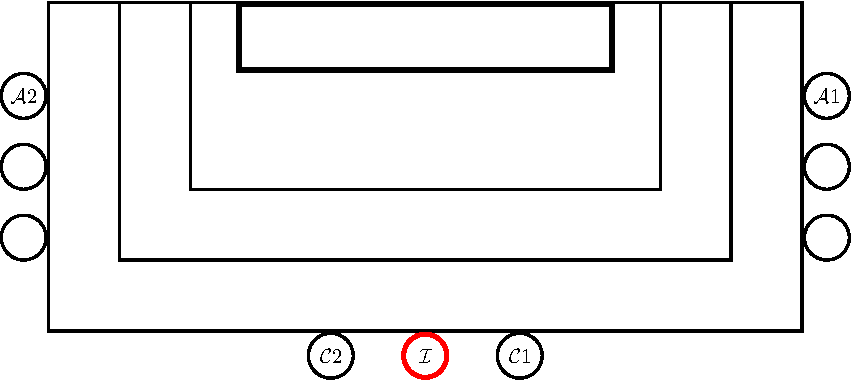
\includegraphics[scale=0.7]{Piatek/Wejscie.pdf}
        \end{figure}
        
        \item \ii~ wraz z ministrantami wykonują skłon, po czym \ii~ pada na twarz, a ministranci klękają na posadce i skłaniają głowy
        \item \ii~ wraz z \cc1 wstają i śpiewana jest modlitwa; ministranci prostują się
        \item po modlitwie wszyscy powstają, robią skłon i udają się na swoje miejsca (\ii, \aa1, \aa2 i \cc~ na sedile)
        \item \cc2 zabiera poduszkę ze stopni ołtarza
        \item \tt~ przynosi pulpit na środek prezbiterium 
        \item wszyscy siadają razem z \ii
        \item śpiewana jest lekcja, po niej następuje responsorium i modlitwa
        \item na \textit{Oremus} wszyscy wstają, na \textit{Flectamus genua} - klękają, na \textit{Levate} - wstają, po skończonej modlitwie - siadają
        \item następuje kolejne czytanie i responsorium
        \item podczas responsorium \tt wynosi pulpit z prezbiterium, a \cc2 przenosi pulpit na stronę Ewangelii i kładzie go na posadce
        \item po responsorium \ii~ odmawia modlitwę przed stopniami ołtarza po czym udaje się do pulpitu i czyta Męke Pańską
        \item ministranci po jej zakończeniu nie mówią \textit{Laus tibi, Christe}
    \end{itemize}

% \section{Uroczyste modły}

    \begin{itemize}
        \item \ii~ wraca do sedilii, wkłada czarną kapę - asystują \cc1 i \cc2
        \item w międzyczasie \aa1 i \aa2 rozpościerają na ołtarzu jeden obrus i \aa1 stawia na środku Mszał
        \item \ii~ z \cc1 i \cc2 udają się do ołtarza (brzegi kapy są podtrzymywane przez \cc1 i \cc2)
        \item podczas modlitw wszyscy stoją, na \textit{Flectamus genua} - klękają, na \textit{Levate} - wstają
    \end{itemize}
    
    



% \section{Adoracja Krzyża}
    
    \begin{itemize}
        \item po modlitwach \ii~ z \cc1 i \cc2 udają się krótką drogą do sedilii, gdzie \ii~ zdejmuje kapę - asystują \cc1 i \cc2
        \item formuje się procesja w kolejności:

        \begin{enumerate}\centering
            \item[] (stopnie ołtarza)
            \item[] \cc2~~~\ii~~~~\cc1
            \item[] \aa2~~~\aa1
        \end{enumerate}
    
        \item uczestniczący w procesji skłaniają się w stronę ołtarza i przechodzą do zakrystii krótką drogą
     
        \item z zakrystii rusza procesja w kolejności:
      
        \begin{enumerate}\centering
            \item[] \cc2~~~\cc1
            \item[] \aa2~~~\ii~~~~\aa1 
            \item[] 
            \item[] gdzie \aa~ trzymają świece, \ii~ - krzyż
        \end{enumerate}
    
        \item procesja długą drogą zmierza stopni ołtarza; po dojściu staje na posadzce po stronie epistoły
     
        \begin{figure}[h]
            \centering
            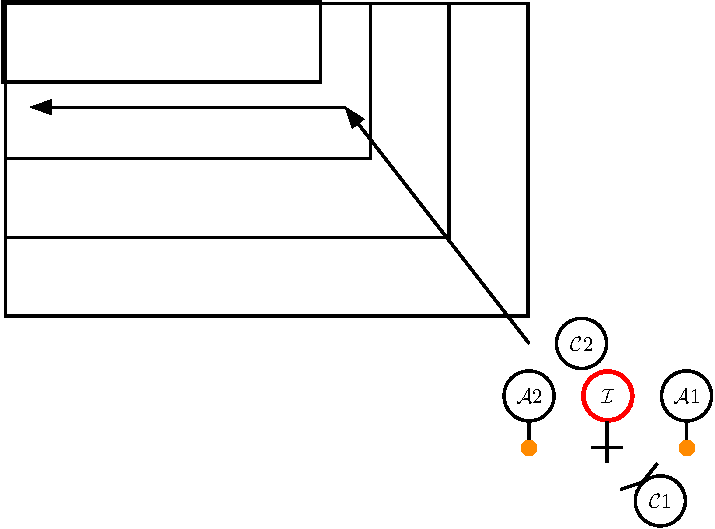
\includegraphics[scale=0.7]{Piatek/Obraz.pdf}
        \end{figure}
     
        \item \ii~ odsłaniając krzyż, śpiewa: \textit{Ecce lignum crucis}, na co wszyscy odpowiadając: \textit{Venite, adoremus} i klękają (ten schemat powtarza się w sumie 3-krotnie)
        \item \aa1 i \aa2 zostawiają akolitki po obu stronach krzyża, po czym odbierają od \ii~ krzyż
        \item \aa2 przynosi poduszkę na stopnie ołtarza; \aa1 i \aa2 kładą na nią krzyż
        \item \cc1 i \aa2 schodzą razem z \ii~ do sedilii i wszyscy ściągają obuwie
      
        \item adoracja następuje w kolejności:
     
        \begin{enumerate}\centering
            \item[] \ii~
            \item[] \cc1
            \item[] \aa2
            \item[] ministranci (dopóki nie przyjdą \aa1 i \aa2)
            \item[] \aa1
            \item[] \aa2 
            \item[] reszta ministrantów
        \end{enumerate}
     
        \item krzyż adorowany będzie przez ministrantów pojedynczo w sposób następujący:
     
        \begin{enumerate}[leftmargin=1cm]
            \item pierwsze przyklęknięcie ma miejsce przy balaskach
            \item drugie - w połowie prezbiterium
            \item trzecie - przy stopniach ołatarza
            \item następuje klęknięcie i pocałunek krzyża
            \item po wstaniu, ministrant wstaje, robi krok w bok, przyklęka z ministrantem, który właśnie doszedł do krzyża  i udaje się na swoje miejsce
            \item wszystkie przyklęknięcia wykonuje się \textbf{w tym samym czasie}, co ministrant przed nami!
        \end{enumerate}
      
        \begin{figure}[h]
            \centering
            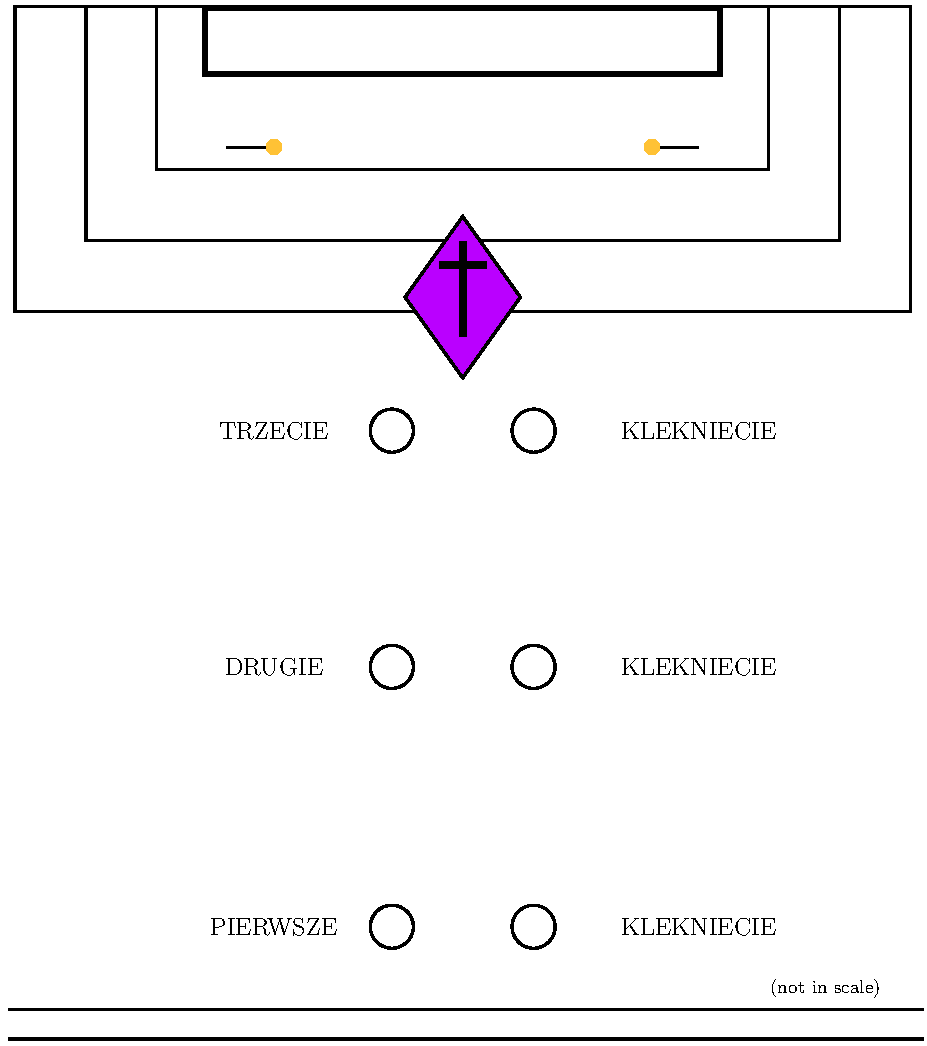
\includegraphics[scale=0.6]{Piatek/Adoracja.pdf}
        \end{figure}
     
        \item \cc1 i \aa2 po dokananiu adoracji, odbierają od \aa1 i \aa2 krzyż i go trzymają
        \item \aa1 i \aa2 po dokonaniu adoracji i nałożeniu butów, klękają po obu stronach krzyża twarzą do siebie na środkowym stopniu ołtarza przy akolitkach  
        \item po skończeniu adoracji przez ministrantów, \cc1 i \aa2 zanoszą krzyż przed prezbiterium w towarzystwie \aa1 i \aa2 ze świecami
        \item \aa1 i \aa2 stwaiają świece po bokach krzyża i odbierają od \cc1 i \aa2 krzyż i go trzymają
        \item po skończonej adoracji \cc1 i \aa2 odbierają od \aa1 i \aa2 krzyż i zanoszą go do stopni ołtarza
        \item tam dołącza do nich \ii~ i wszyscy trzej wchodzą po stopniach i \ii~ umieszcza krzyż na tabernakulum
        \item w międzyczasie \aa1 i \aa2 biorą swoje świece i stawiają je na ołtarzu
    \end{itemize}
    

% \section{Obrzęd Komunii Św.}

    \begin{itemize}
     \item \ii~ zmienia szaty - asystuje \cc1
     \item \ii~ zanosi korporał na ołtarz w towarzystwie \cc1 i \cc2
     \item \aa1 i \aa2 ustawiają się przed stopniami ołtarza i wraz z \oo~, \cc1, \cc2 i \ii~ procesyjnie udają się to ołtarza przechowywania 
     \item podczas powrotu procesji do ołtarza, \cc1 i \cc2 uderzają kołatką, a wszyscy ministranci klęczą
     \item po dojściu do stopni ołatarza \oo~ odchodzi na bok, \aa1 i \aa2 odkładają akolitki na ołtarzu, a \cc1, \cc2 i \ii~ podchodzą do ołarza
     
     \begin{figure}[h]
     \centering
        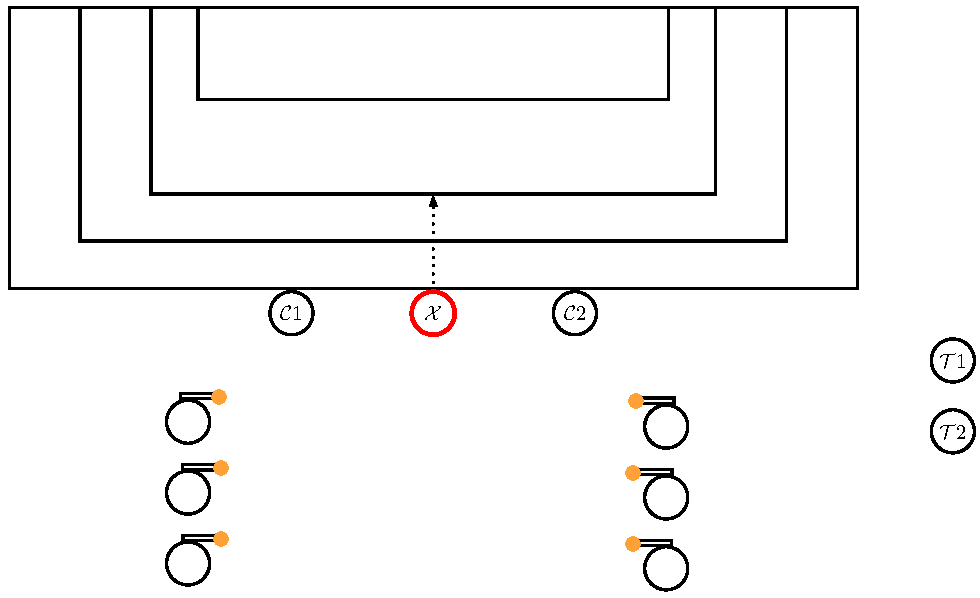
\includegraphics[scale=0.6]{Piatek/NSakrament.pdf}
     \end{figure}
     
     \item przy ołtarzu \cc2 odbiera welon, po czym przyklęka i idzie na swoje miejsce
     \item wszyscy ministranci wstają; w odpowiednim momencie za \ii~ odmawiają \textit{Pater noster}
     \item na znak \cc1 ministranci ustawiają się parami na posadzce do przyjęcia Komunii i na kolejny znak - klękają
     \item w tym czasie \aa1 (z obrusem komunijnym) i \aa2 klękają twarzami do siebie na najwyższym stopniu ołtarza
     \item \cc1 rozpoczyna \textit{Confiteor}, do którego dołączają się pozostali
     \item po \textit{Indulgentiam...} \aa1 i \aa2 rozciągają obrus komunijny między sobą
     \item pierwsi do Komunii przystępują ministranci od pateny i świeczki sanctusowej; zaraz po jej przyjęciu asystują \ii~
     \item do Komunii ministranci przystępują w następujący sposób (więcej: \hyperref[komunia]{patrz Dodatek}):
     
      \begin{enumerate}[leftmargin=1cm]
       \item para przyklęka na posadzce równocześnie z poprzedzającą ją parą
       \item po wejściu na stopnie ołtarza, klęka na najwyższym stopniu
       \item przyjąwszy Komunię, przyklęka w miejscu i udaje się na swoje miejsce
      \end{enumerate}
    
     \item po przyjęciu Komunii św. przez ministrantów, \aa1 i \aa2 wstają i udają się z obrusem komunijnym do balasek; razem z nimi przechodzą \cc1 i \cc2
     \item po skończonej Komunii wiernych, \aa1 i \aa2 składają obrus komunijny i odkładają na kredensji i przy niej pozostają
     \item wszyscy wstają, gdy zostanie schowany Najświętszy Sakrament i pozostają w tej pozycji
     \item gdy \ii~ oczyści patenę, zabiera ją \aa1; korporał nie jest chowany!
     \item \ii~ śpiewa trzy modlitwy po komuni; po nich \cc2 zamyka i ściąga z ołtarza mszał
     \item \ii~ udaje się do sedilii i zmienia szaty - asystuje \cc1
    \end{itemize}



% \section{Procesja do Bożego Grobu}

	\begin{itemize}
	 \item \tt1 i \tt2 wychodzą z kadzielnicami, \oo~ - z ombrelino, \ding{63} staje z krzyżem procesyjnym u wejścia do prezbiterium
	 \item ministranci zapalają swoje świece
	 \item \aa1 przynosi na ołtarz monstrancje i przejrzysty welon do niej
	 \item \ii~ wraz z \cc1 i \cc2 udaje się do stopni ołtarza i sam wchodzi na górę
	 \item po wystawieniu Najświętszego Sakramentu \ii~ schodzi po stopniach, zasypuje kadzidło i okadza N. S.
	 \item po okadzeniu \cc2 nakłada \ii~ welon naramienny i wraca na miejsce
	 \item \aa1 i \aa2 z akolitkami (wziętymi z kredensji) dołączają do \ding{63}
	 \item \cc1 i \cc2 biorą kołatki 
	 \item gdy \ii~ bierze monstrancję, formuje się procesja w kolejności:
	 
	  \begin{enumerate}\centering
	   \item[] (stopnie ołtarza)
	   \item[] \cc2~~~\ii~~~~\oo~~~~\cc1
	   \item[] \tt1~~~\tt2
	   \item[] chór ze świeczkami (parami)
	   \item[] \aa2~~~\ding{63}~~~\aa1
	   \end{enumerate}
	  
	  \newpage
	  
	 \begin{figure}[h]
	 \centering
	    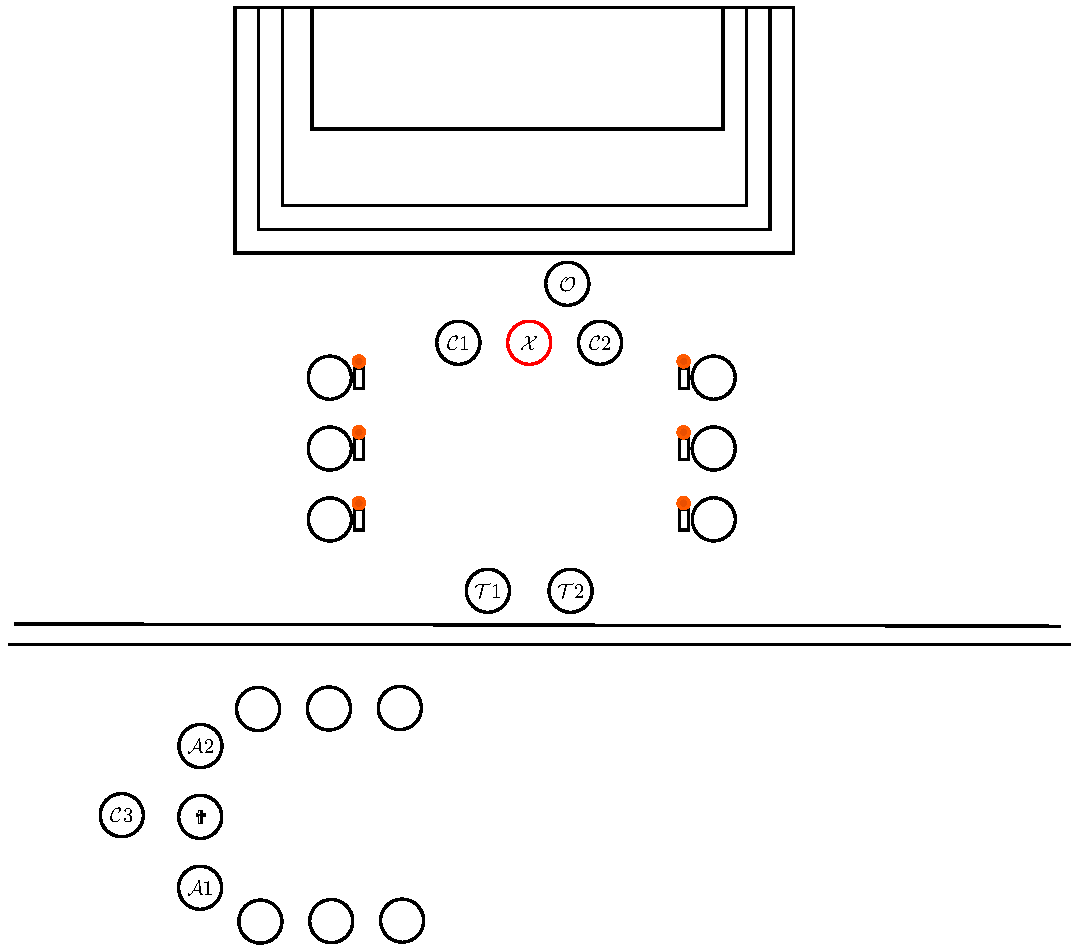
\includegraphics[scale=0.6]{Piatek/Procesja1.pdf}
	 \end{figure}
	 
	 \item po dokonaniu wystawienia w Bożym Grobie następuje zasypanie i okadzenie oraz krótka adoracja
	 
	 \begin{figure}[h]
	 \centering
	    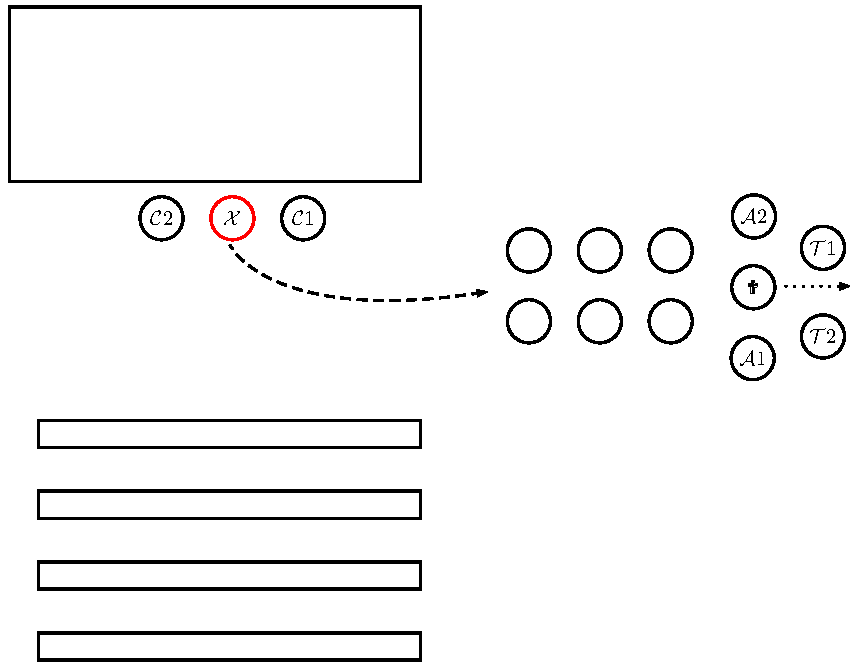
\includegraphics[scale=0.7]{Piatek/Procesja2.pdf}
	 \end{figure}
	 
	 \item procesja udaje się do zakrysti
	\end{itemize}



% \section{Dodatek}
  \subsection{Przyjmowanie Komunii Św. - z instrukcji M. Rumina}
  \label{komunia}

    \begin{itemize}
      \item na znak \cc1 \aa1 bierze z kredencji obrus komunijny, razem z \aa2 klękają pośrodku, wchodzą na najwyższy stopień ołtarza i klękają twarzami do siebie (jeszcze nie rozkładają obrusu)
      \item ministranci biorący udział w lucenarium wchodzą dwójkami do prezbiterium, tworząc w ten sposób naturalną „kolejkę” do Komunii św. Przed nimi do kolejki wchodzą księża, klerycy  \footnote{W Wielki Piątek najprawdopodobniej nie będzie żadny kleryków ani księży. W takim razie wzmianki o nich pomijamy, a na rysunkach w ich miejsce wstawiamy pustą przestrzeń} i \cc1, za nimi reszta ministrantów z chóru. \cc1 – zależnie od ilości duchownych i ministrantów może staje do komunii sam lub w parze
      \item po \textit{Indulgentiam} rozkładany jest obrus komunijny 
      
      \begin{figure}[h]
      \centering
	  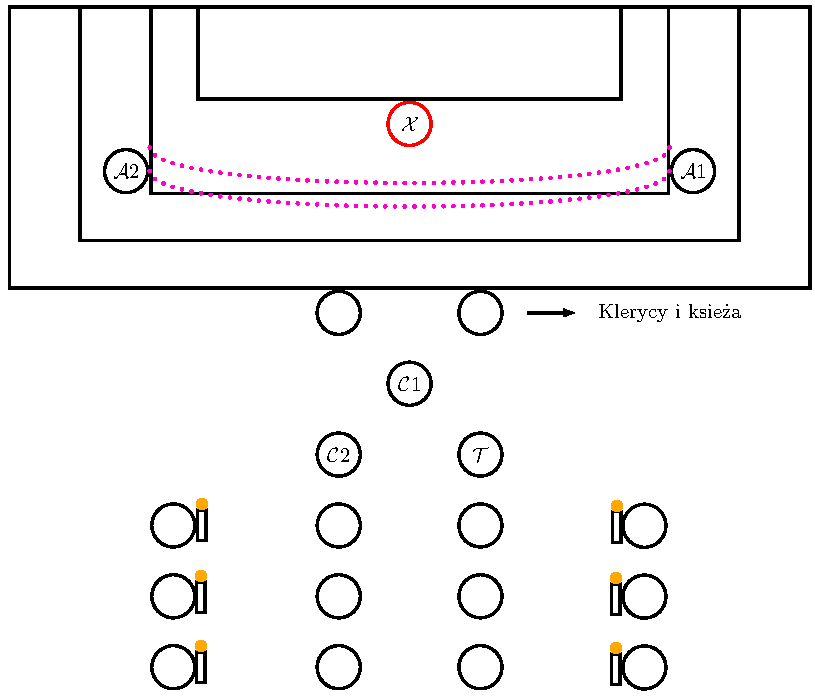
\includegraphics[scale=0.5]{Piatek/Komunia1.pdf}
      \end{figure}
    
      \item \cc1 podaje patenę pierwszemu duchownemu przyjmującemu Komunię św., albo jeśli nie ma duchownych trzyma ją sam. Po przyjęciu Komunii Św. zajmuje miejsce przy \ii~, gdzie asystuje z pateną
      \item \cc2 lub \tt~ po przyjęciu Komunii św. zajmuje miejsce przy celebransie ze świeczką sanctusową
    
      \begin{figure}[h]
      \centering
	  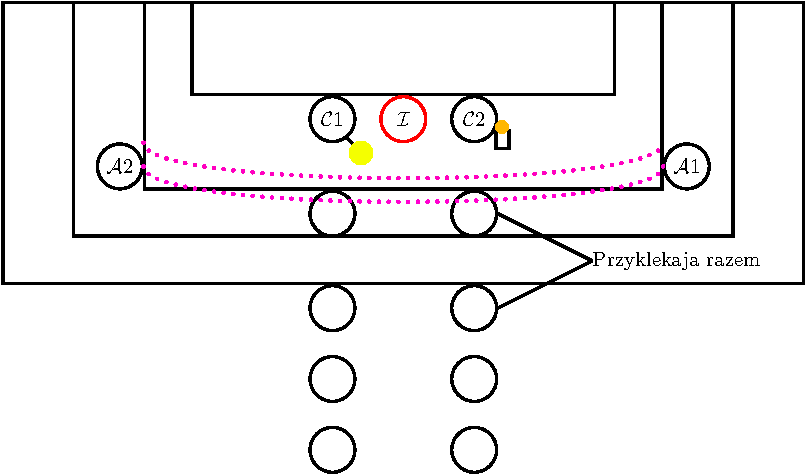
\includegraphics[scale=0.5]{Piatek/Komunia2.pdf}
      \end{figure}
      
      \item \aa1 i \aa2 trzymający obrus przyjmują Komunię św. razem z \cc1
      \item każda dwójka przystępująca do Komunii św. przyklęka \textbf{jednocześnie z poprzedzającą parą}, wchodzi na stopnie i klęka na dwa kolana. Po przyjęciu komunii znów przyklęka jednocześnie z parą stojącą za nimi. Ze stopni ołtarza schodzimy w lewo – do chóru.
      \item po przyjęciu Komunii Św. przez ministrantów \aa1 i \aa2 wstają i przechodzą do miejsca udzielalnia komunii wiernym. Z pateną i świeczką sanctusową asystują \cc1 i \cc2
      
      \begin{figure}[h]
      \centering
	  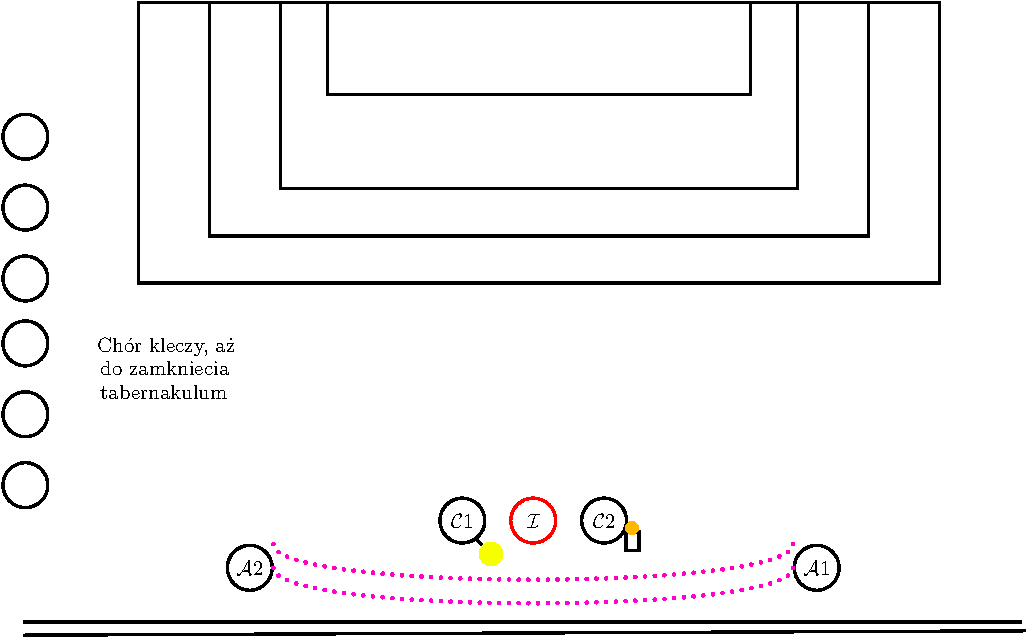
\includegraphics[scale=0.5]{Piatek/Komunia3.pdf}
      \end{figure}
    
    \end{itemize}
    
    \newpage

\section{Do poprawy}
  \begin{itemize}
    \item Sprawdizć wcześniej czy są poprawne modlitwy na Żydów w OHS-ie
    \item Wybrać kompetentnych ministarntów do pateny i świeczki sanktusowej lub niech robią to ceremoniarze
  \end{itemize}

% \newpage

% \chapter{Wigilia Paschalna}

	\section{Przygotowanie do obrzędów}

		\subsection{Ołtarz główny}
		
			\begin{itemize}
				\item narazie pusto
			\end{itemize}

% \section{Liturgia światła}
	
	\begin{itemize}
		\item Do poświęcenia ognia wychodzimy nastąpująco:
		\begin{itemize}
			\item \tt~ z pustą kadzielnicą, 
			\item \ding{64},
			\item \aa1 z kropidłem, 
			\item \aa2 z tacką z granami i rylcem,
			\item \mm1 z paschałem, 
			\item \cc2 trzymając w ręku dalmatykę i stułę, 
			\item \cc1 z kropidłem i OHS, 
			\item \ii~ w kapie.
		\end{itemize}
		\item turyfer po dojściu do ogniska od razu wrzuca do środka węgielki, aby się rozpaliły.
		\item stajemy przed kościołem w następujących pozycjach:
		\item (tutaj będzie obrazek)
		\item następuje oświęcenie ognia -- modlitwa
		\item potem pokropienie ogniska -- \aa1 podaje kropidło bezpośrednio \ii~ i potem je odbiera Także i on przytrzymuje kapę, aby się \textbf{nie spaliła}.
		\item po poświęceniu ogniska \tt~ nakłada do trybularza węgiel, następnie zasypanie i okadzenie. Teraz turyfer trzyma kapę, aby się \textbf{nie spaliła}.
		\item jeden z kantorów odpala od ogniska świeczkę i idzie z nią do kościoła (może to być M. Rumin)
		\item następnie naprzeciwko \ii~ staje \mm z paschałem. Po jego lewej staje \aa2 z
		tacką z rylcem. \ii~ kreśli wszystkie litery i cyfry.
		\item poświęcenie gran: trzykrotne pokropienie i okadzenie (\aa1 I podaje i odbiera kropidło, \tt~ podaje trybularz: bez zasypania!)
		\item włożenie wszystkich gran w paschał.
		\item \cc1 odpala świeczkę od ognia i podaje \ii. Ten odpala paschał i potem go błogosławi.
		\item \ii~ przebiera się w białą stułę i dalmatykę. Pomaga mu w tym \cc2 oraz \aa2.
		\item dopiero teraz nastepuje zasypanie.
		\item procesja z paschałem do kościoła: \tt, \ding{64}, \ii~ z paschałem, \cc,
		\aa i \mm1, który zabiera tackę i kropidło.
		\item trzykrotne Lumen Christi: zaraz po wejściu do kościoła na stopniu koło figury św. Jadwigi,
		potem w połowie nawy głównej (tam gdzie siedzą wierni) i w prezbiterium.
		\item UWAGA! Tu zmiana w stosunku do lat poprzednich. Zawsze wchodziliśmy do kościoła i skręcaliśmy w prawo. Tym razem w lewo. Uznałem, że paschał ma się kierować bezpośrednio do prezbiterium, a nie być obnoszony w procesji dookoła kościoła.
	\end{itemize}
	
	

% \section{Liturgia słowa}
	
		\begin{itemize}
			\item po przybyciu do prezbiterium stajemy następująco:
			\item (tutaj będzie grafika)
			\item następuje zasypanie, potem \cc~ odmawia modlitwę, okadzenie księgi i
			\textit{Exsultet} 
			\item \aa~ biorą z kredensu świeczki i odpalają sobie, podobnie \mm1
			\item \cc2 na słowa \textit{O vere beata nox...} zapala lampy w prezbiterium.
			\item po orędziu paschalnym \cc2 wraz z \aa2 pomagają \ii~ przebrać się z powrotem w kapę
			\item następnie \cc~ odnosi dalmatykę do zakrystii i wraca na swoje miejsce razem z drugim OHS
			\item \cc1 zabiera z pulpitu białą narzutkę i kładzie na pulpicie teksty proroctw 
			\item \ding{63} odnosi krzyż za ołtarz
			\item \tt~ odnosi kadzielnicę i wraca na swoje miejsce
			\item siedzimy w prezbiterium następująco:
			\item (tutaj będzie odpowiednia grafika)
			\item następują proroctwa
			\item po trzecim proroctwie \tt~ idzie po kadzielnicę i bokiem przemyka w stronę chrzcielnicy i zapala tam światła
		\end{itemize}

% \section{Liturgia chrzcielna}

	\begin{itemize}
		\item po ostatnim proroctwie:
			\begin{itemize}
				\item \aa1 odpala od paschału akolitki
				\item \ii wraz z \cc klęka po stronie lekcji na pierwszym stopniu
				\item \ding{63} idzie po krzyż procesyjny
			\end{itemize}
		\item gdy \ii uklęknie kantorzy zaczynają śpiew \textit{Litanii do Wszystkich Świętych}
		\item w tym czasie ustawiamy procesję do chrzcielnicy:
			\begin{itemize}
				\item \mm1 z \textbf{zapalonym} paschałem
				\item \ding{63} w towarzystwie \aa
				\item pozostali ministranci i kantorzy
			\end{itemize}
		\item procesja rusza po słowach \textit{Sancta Trinitas Unus Deus: miserere nobis}
		\item (tutaj będzie rysunek)
		\item po dojściu do chrzcielnicy kantorzy śpiewają kantyk \textit{Sicut Cervus} i dopiero po nim zaczyna się poświęcenie wody chrzcielnej
		\item stoimy w następującym porządku:
		\item (tutaj będzie obrazek)
		\item następuje modlitwa \textit{Omnipotens sempiterne Deus, respice}
		\item następnie druga modlitwa i poświęcenie wody (jak zwykle)
		\item potem zasypanie i okadzenie wody chrzcielnej
		\item zamiana kapy fioletowej 
		\item odnowienie przyrzeczeń chrzcielnych (przy chrzcielnicy) i pokropienie
		\item na pokropienie chór śpiewa stosowną pieśń (np.\textit{Przez chrztu świętego wielki dar})
		\item oleje i kapa biała leżą przygotowane na stoliku, podobnie kociołek na wodę święconą oraz garnek na nią, aby wierni mogli sobie jej więcej nabrać do domu
		\item \cc1 podaje \ii~ oleje
		\item \cc2 po nabraniu wody do kociołka i do garnka ucieka z pola widzenia bokiem i zaczyna przygotowywać prezbiterium do Mszy (jeszcze jak reszta jest w chrzcielnicy). Trzeba odstawić stojak na paschał na stronę ewangelii, odstawić pulpit, powiesić stułę na krzyż, ustawić relikwie, kwiaty. Na razie nie rozkładać obrusów!!! 
		\item po okadzeniu wody chrzcielnej \tt~ też od razu ucieka bokiem i idzie pomagać \cc2
		\item po skończonych odnowieniach ustawiamy procesję z powrotem do Ołtarza w tym samym porządku co poprzednio
		\item kantorzy intonują drugą część \textit{Litanii do Wszystkich Świętych}
		\item po przybyciu do Ołtarza \mm1 odstawia Paschał na swoje miejsce
		\item \cc1 zapala od paschału świece na Ołtarzu i rozkłada obrusy -- pomaga mu \mm1
		\item \cc2 zamienia się z \cc1 miejscami i klęka z \ii~ po stronie lekcji na stopniu
		\item \aa~ wraz z \ding{63} stoją przy kredensie
		\item kantorzy klękają na stopniach prezbiterium i kontynuują litanię
		\item \tt~ idzie już bokiem do zakrystii i przebiera się
		\item po wezwaniu \textit{Peccatores} \ii~ wstaje i wraz ze wszystkimi udaje się do zakrystii, gdzie zmieniamy komże na ładniejsze, \ii~ ubiera ornat biały.
	\end{itemize}
	

% \section{Msza Św. i procesja do Bożego Grobu}

	\subsection{Msza Św.}

	\begin{itemize}
		\item po przebraniu się od udajemy się procesyjnie do Ołtarza i rozpoczyna się Msza św. 
		\item nie ma modlitw u stopni Ołtarza, nie ma Confiteor, Od razu Aufer a nobis 
		\item zasypanie i okadzenie
		\item \aa1 niech ma	na uwadze, że nie musi Mszału zabierać z Ołtarza, bo ten jest na stoliku; ale trzeba go po okadzeniu ustawić na ołtarz
		\item \cc2 posługuje przy Ołtarzu; teraz on jest ważniejszy
		\item \aa~ na \textit{Gloria} dzwonią dzwonkami; w tym czasie w sygnaturkę uderza \tt~ i \cc1
		\item Msza biegnie normalnie; \cc1 idzie w tym czasie do chrzcielnicy i sprząta co nieco.
		\item przed komunią (po przyjęciu komunii przez \ii) \cc2 zaczyna \textit{Confiteor}!!!
		\item po komunii są \textit{Laudesy}. Pamiętamy, że na słowa \textit{Benedictus} żegnamy się znakiem krzyża
		\item potem	jest zasypanie i okadzenie ołtarza, \ii, usługujących i wiernych (jak w trkacie ofiarowania)
		\item po \textit{Ite missa est, alleluia, alleluia} i błogosławieństwie nie ma ostatniej ewangelii. 
		\item \ii~ przebiera ornat na kapę
		\item potem procesyjnie udajemy się do Grobu. 
		\item \cc2 zabiera ze sobą dzwonki
		\item \cc1 przygotuje Ołtarz i za chwilę dojdzie do reszty.
	\end{itemize}

	\subsection{Przy Grobie}
	
	\begin{itemize}
		\item ustawiamy się następująco:
		\item (tutaj będzie rysunek)
		\item wszyscy klękamy
		\item \ii intonuje \textit{Gloria, tibi Trinitas}
		\item po skończeniu modlitw \mm1 wstaje i bierze figurę Zmartwychwstałego i staje obok \ding{63}
		\item procesja rusza jak tylko rozpocznie się śpiew pieśni po polsku i wygląda następująco:
		\item (tutaj obrazek)
		\item po przybyciu do Ołtarza, \aa~ i \ding{64} stają przy kredensie, \mm1 ustawia figurę zmartwychwstałego po stronie ewangelii i schodzi na swoje miejsce, \tt~ staje po swojej stronie, \cc2 staje u stopni Ołtarza po prawej stronie \ii, a \cc1 jak już odstawi parasolkę to staje po lewej stronie \ii
		\item śpiewamy na stojąco \textit{Te Deum}
		\item potem jest błogosławieństwo (nie ma podnoszenia krzyża, nie ma
		\textit{Przed tak wielkim sakramentem})
		\item na koniec \ii intonuje \textit{Regina Caeli}, odmawia modlitwę i po
		tym schodzimy procesyjnie do zakrystii
	\end{itemize}

	\bigskip

	\begin{center}
		\Large
		\textbf{Wesołych Świąt Zmartwychwstania Pańskiego!}
	\end{center}
	










	

% \section{Procesja do Bożego Grobu}

\begin{itemize}
	\item \tt1 i \tt2 wychodzą z kadzielnicami, \oo~ - z ombrelino, \ding{63}
	      staje z krzyżem procesyjnym u wejścia do prezbiterium
	\item ministranci zapalają swoje świece
	\item \aa1 przynosi na ołtarz monstrancje i przejrzysty welon do niej
	\item \ii~ wraz z \cc1 i \cc2 udaje się do stopni ołtarza i sam wchodzi na
	      górę
	\item po wystawieniu Najświętszego Sakramentu \ii~ schodzi po stopniach,
	      zasypuje kadzidło i okadza N. S.
	\item po okadzeniu \cc2 nakłada \ii~ welon naramienny i wraca na miejsce
	\item \aa1 i \aa2 z akolitkami (wziętymi z kredensji) dołączają do \ding{63}
	\item \cc1 i \cc2 biorą kołatki
	\item gdy \ii~ bierze monstrancję, formuje się procesja w kolejności:

	      \begin{enumerate}\centering
		      \item[] (stopnie ołtarza)
		      \item[] \cc2~~~\ii~~~~\oo~~~~\cc1
		      \item[] \tt1~~~\tt2
		      \item[] chór ze świeczkami (parami)
		      \item[] \aa2~~~\ding{63}~~~\aa1
	      \end{enumerate}

	      \newpage

	      \begin{figure}[h]
		      \centering
		      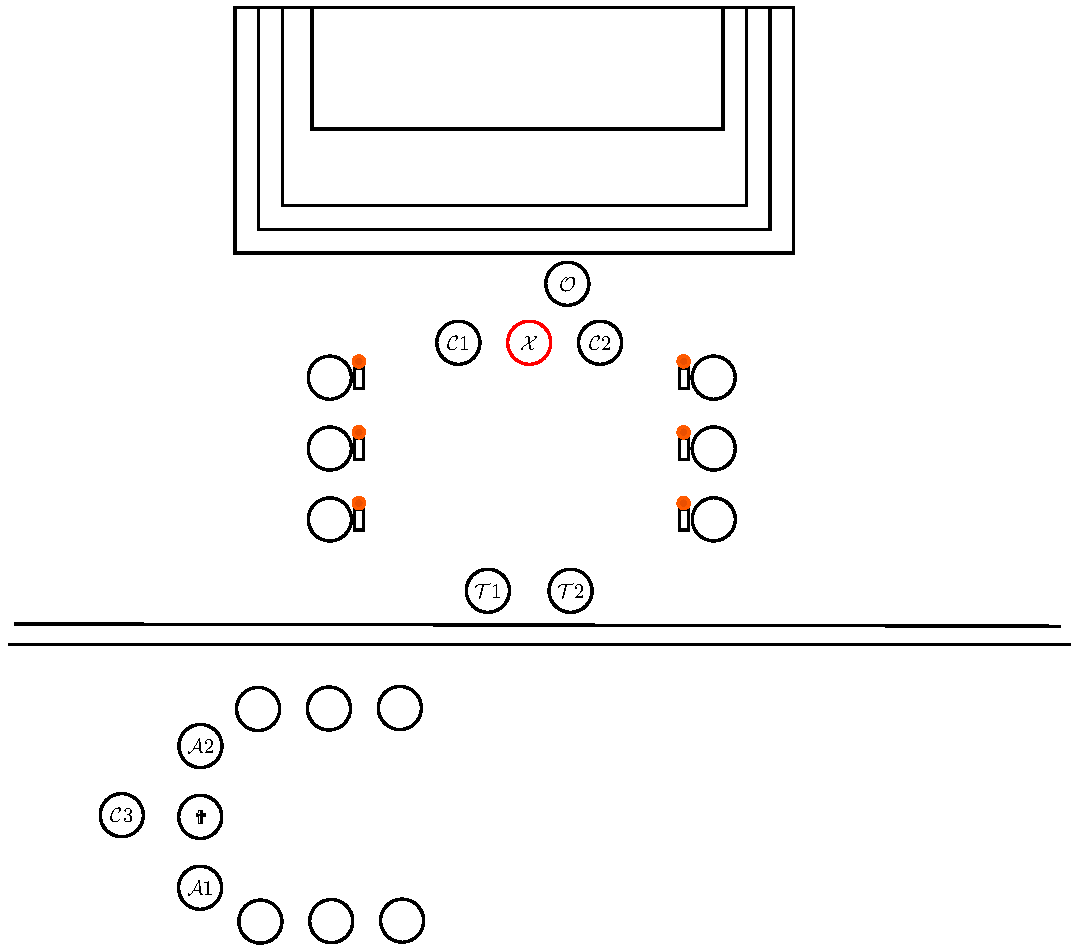
\includegraphics[scale=0.6]{Piatek/Procesja1.pdf}
	      \end{figure}

	\item po dokonaniu wystawienia w Bożym Grobie następuje zasypanie i
	      okadzenie oraz krótka adoracja

	      \begin{figure}[h]
		      \centering
		      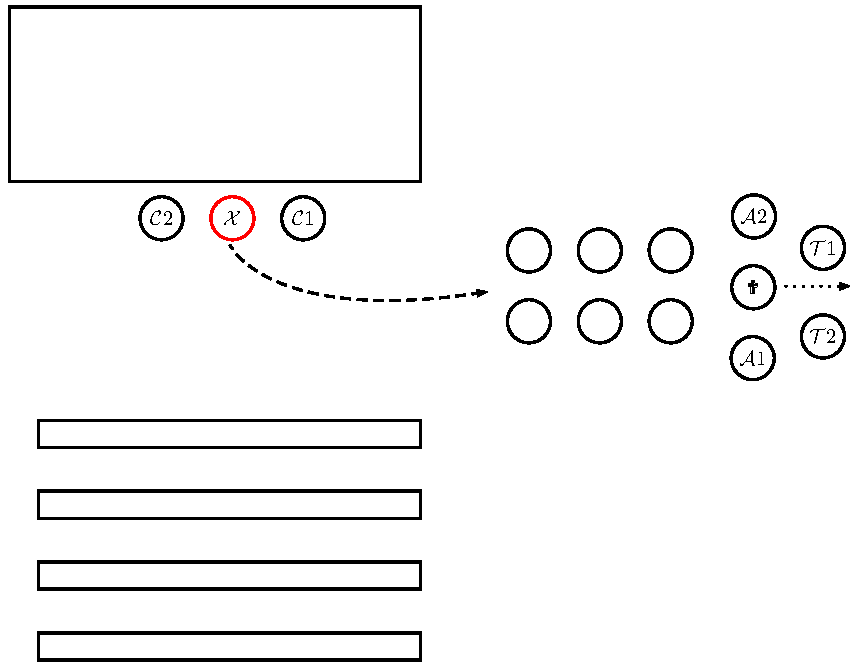
\includegraphics[scale=0.7]{Piatek/Procesja2.pdf}
	      \end{figure}

	\item procesja udaje się do zakrysti
\end{itemize}



\end{document}
